\documentclass{report}
\usepackage[utf8]{inputenc}
\usepackage[a4paper, margin=1in]{geometry}
\usepackage{amsmath}
\usepackage{amssymb}
\usepackage{graphicx}
\usepackage{url}
\usepackage{hyperref}
\newcommand{\algorithmautorefname}{Algorithm}
\usepackage{algorithm}
\usepackage[noend]{algpseudocode}
\usepackage{subcaption}

\linespread{1.5}

\renewcommand{\algorithmicforall}{\textbf{for each}}
\newcommand{\algorithmicbreak}{\textbf{break}}
\newcommand{\Break}{\State \algorithmicbreak}
\newcommand{\Continue}{\State \textbf{continue}}
\renewcommand{\Comment}[1]{\hfill\textit{$\triangleright$ #1}}

\title{Selected Methods in $N$-body Simulations}
\author{Aleksy Bałaziński}
\date{\today}

\begin{document}

\newcommand{\PThreeM}{P$^3$M}

\begin{titlepage}
    \centering
    \vspace*{2cm}

    {\Huge\bfseries Selected Methods in $N$-body Simulations\par}
    \vspace{1.5cm}

    {\Large\bfseries Aleksy Bałaziński\par}
    \vspace{1.5cm}

    {\large
        A thesis submitted in partial fulfillment of the requirements\\
        for the degree of\\
        \textbf{Master of Science in Engineering}\\
        in \textbf{Applied Computer Science}\par
    }
    \vspace{0.5cm}

    {\large
        Faculty of Electrical Engineering\\
        Warsaw University of Technology
        \par}

    \vfill

    {\large \today\par}
\end{titlepage}

\tableofcontents


\chapter{Introduction}
The dominant force over large distances is the gravitational force.
It controls the motion of planets in the solar system and is responsible for the evolution of stars and galaxies, and the whole cosmos \cite{nordtvedt2025gravity}.
Although the motion of two bodies orbiting each other lends itself to an analytical description, no general solution for systems comprising three or more bodies is known.
Therefore, the importance of numerical simulations of many-body systems (usually referred to as \textit{N-body simulations}) is hard to overestimate.

Even though the direct beneficiary of advances in the area of $N$-body simulations is the field of astrophysics, the development of such tools is highly interdisciplinary in nature.
The theory behind algorithms that make fast simulations of this type possible is often mathematically involved and requires a good grasp of general physics.
On the other hand, efficient implementation of these ideas demands proficiency in computer science, particularly in areas such as data structures, parallel computing, and performance optimization.
Consequently, the development of $N$-body simulation codes is challenging but also intellectually rewarding.

\section{Problem statement}
To better understand the computational challenge before us, we begin by formulating the physical setup.
The force exerted on a body with mass $m_2$ at the point $\mathbf{x}_2$ by a body with mass $m_1$ located at $\mathbf{x}_1$ can be expressed by the relation
\begin{equation}\label{eq:law-of-uni-grav}
    \mathbf{F} = -G\frac{m_1m_2}{|\mathbf{x}_{21}|^3}\mathbf{x}_{21}
\end{equation}
where $G$ is the gravitational constant $6.674\times 10^{-11}\, \mathrm{m}^3 \,\mathrm{kg}^{-1}\,\mathrm{s}^{-2}$ and $\mathbf{x}_{21} = \mathbf{x}_2 - \mathbf{x}_1$.
Therefore, the evolution of a system of $N$ bodies is governed by $N$ equations
\begin{equation}\label{eq:pp-method}
    \ddot{\mathbf{x}}_i = -G\sum_{j\neq i} \frac{m_j}{|\mathbf{x}_{ij}|^3}\mathbf{x}_{ij}.
\end{equation}
for each $i = 1,\dots, N$.
Direct application of \autoref{eq:pp-method} is the basis of the so-called \textit{particle-particle} method.
The method is characterized by $O(N^2)$ time complexity (more precisely, it requires $(N-1)N/2$ operations if Newton's 3rd law is used in the computation).
This running time characteristic $T(N)$ (running time of one simulation iteration) can be directly observed by running an implementation of the method (see \autoref{fig:pp-method-scaling}).
\begin{figure}[htp]
    \centering
    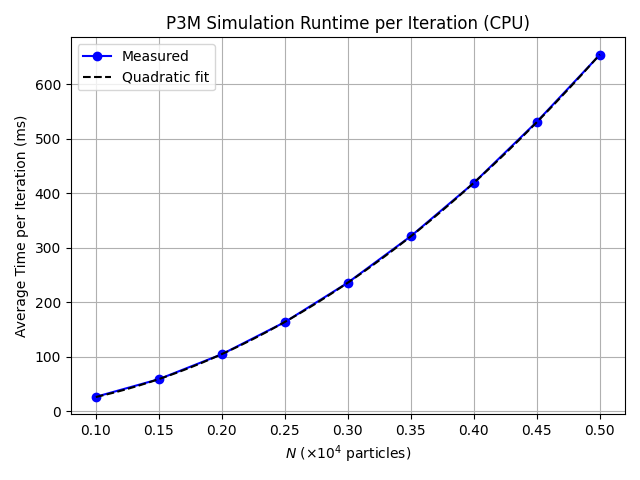
\includegraphics[scale=0.5]{chapters/introduction/img/pp_time.png}
    \caption{Scaling of the PP method.}
    \label{fig:pp-method-scaling}
\end{figure}
The exact form of $T(N)$ depends on the implementation details and the type of hardware used, but assuming that the code whose running time is shown in \autoref{fig:pp-method-scaling} is not tragically inefficient, we can draw some general conclusions regarding the applicability of the PP method.
Fitting a quadratic through the points shown in the figure reveals the following approximation: $T(1{,}000N) \approx 26.1N^2 + 0.32N$ [ms].
In a reasonable particle simulation, one often deals with tens of thousands of particles (if not more) and the simulation can span hundreds of iterations.
Thus, assuming sensible values of $N = 50{,}000$ and 200 iterations, we get the expected running time of $\approx 3.5$ hours!
This clearly shows that more efficient algorithms have to be put in place.

\section{Historical development}\label{sec:historical-development}
The \textit{particle-mesh} (PM) technique, introduced by Roger W. Hockney and James W. Eastwood, was a significant improvement over the PP method.
In the PM approach, the space is divided into a rectangular grid (or mesh) of cells.
Each cell is assigned a portion of the mass of nearby particles, creating a density distribution $\rho(\mathbf{x})$.
The relation between the density and the gravitational potential $\phi$, in the form of Poisson's equation
\begin{equation}\label{eq:poisson}
    \nabla^2\phi = 4\pi G \rho,
\end{equation}
is then used to obtain the potential at each cell center using Fourier techniques.
The gravitational field $\mathbf{g}$ can then be calculated as $\mathbf{g} = -\nabla \phi$.
Since $\mathbf{g}$ equals the acceleration due to gravity, we get $\ddot{\mathbf{x}}_i = \mathbf{g}(\mathbf{x}_i)$.
The PM method and its theoretical grounding were most extensively described by Hockney and Eastwood in \textit{Computer Simulation Using Particles} textbook published in 1988 \cite{Hockney1988}.
However, one of the first papers treating the problem of solving the Poisson equation using Fourier analysis (\textit{A Fast Direct Solution of Poisson's Equation Using Fourier Analysis} by R.W. Hockney) can be traced back to 1965 \cite{10.1145/321250.321259}.

The drawback of the PM method is its poor modeling of forces over short distances.
Eastwood and Hockney proposed a remedy for this problem in the form of a hybrid approach, called the \textit{particle-particle-particle-mesh} method (or \PThreeM{} in short).
In the \PThreeM{} method, the force on a given particle is split into two components: \textit{short-range} and \textit{long-range} force.
The long-range force is calculated using the PM method, whereas the short-range force can be found by direct summation of the forces due to nearby particles.
The \PThreeM{} method was developed across the papers published by the authors between 1973 and 1980 with its thorough description given in \textit{Computer Simulation Using Particles} \cite{Hockney1988}.

The computational complexity of the PM and \PThreeM{} methods depends on the implementation of the potential solver used to calculate $\phi$ from \autoref{eq:poisson}.
For instance, if a fast Fourier transform is used, then the complexity of the PM algorithm is $O(N + N_g^3\log N_g^3)$, where $N_g$ is the number of cells in a single dimension of the grid (note that it is linear in $N$).
For the \PThreeM{} method, the worst-case scenario happens when all particles are clustered closely together, which causes the short-range $O(N^2)$ correction part to become dominant.

In 1986, Josh Barnes and Piet Hut introduced a hierarchical method for $N$-body simulations, now known as the Barnes-Hut algorithm, in the paper \textit{A hierarchical O(N log N) force-calculation algorithm} \cite{barnes1986hierarchical}.
The method developed by the authors uses a hierarchical subdivision of space into cubical cells where the subdivision is carried out recursively until at most one body can be found in any subdivision.
The algorithm reduces the time complexity to $O(N \log N)$ by approximating groups of distant particles as a single ``pseudo-particle.''

Other notable examples of $N$-body simulation algorithms include (and are not restricted to) the Fast Multipole Method and Adaptive Mesh Refinement method \cite{trenti2008nbody}.

\section{Aim and scope}
This thesis has three main goals:
\begin{enumerate}
    \item To develop a program implementing the PM, \PThreeM{}, and Barnes-Hut algorithms focusing on correctness and performance;
    \item To introduce these algorithms and analyze their strengths and weaknesses through error analysis and performance benchmarks using our implementation;
    \item To implement simple astronomical system models to test and evaluate the methods.
\end{enumerate}
The field of $N$-body simulations has been extensively studied (see \autoref{sec:historical-development}), making novel contributions challenging.
However, since our implementation is written from scratch, we aim to provide practical insights via:
\begin{enumerate}
    \item Comparing GPU and CPU implementations of the PM method;
    \item Parallelizing the short-range correction in the \PThreeM{} method;
    \item Implementing a cache-friendly tree construction for the Barnes-Hut algorithm.
\end{enumerate}
The complete source code, including all algorithms and simulation models, is available at \url{https://github.com/AleksyBalazinski/ParticleSimulation}.

\chapter{Particle-mesh method} % checked
The particle-mesh method can be described as the following sequence of four steps:
\begin{enumerate}
    \item Assign masses to mesh points,
    \item Solve the field equation (\autoref{eq:poisson}) on the mesh,
    \item Calculate the field strength at mesh-points,
    \item Find forces applied to individual particles by interpolation.
\end{enumerate}
In this section, each of these steps will be described in more detail.

\section{Mass assignment}\label{sec:mass-assignment}
The specifics of assigning mass from particles to mesh points depend on the density profile (or \textit{shape}) associated with the particles.
In general, the particles need not be represented as idealized dimensionless points;
indeed, it is possible to construct a hierarchy of shapes where each successive member covers a larger number of mesh points and whose application leads to smaller numerical errors.

An infinite hierarchy of shapes with this property, as described by Hockney and Eastwood in \cite{Hockney1988}, can be generated by successive convolutions with the ``top-hat'' function $\Pi$, defined as
\begin{equation*}
    \Pi(x) = \begin{cases}
        1,           & |x| < \frac{1}{2} \\
        \frac{1}{2}, & |x| = 1           \\
        0,           & \text{otherwise}.
    \end{cases}
\end{equation*}
The three most popular assignment schemes that hail from this family (and the ones implemented in our program) are the \textit{nearest grid point} (NGP), \textit{cloud in cell} (CIC), and \textit{triangular shaped cloud} (TSC) schemes, with shapes $S$ given by
\begin{align*}
    S_\text{NGP} & = \delta(x), & S_\text{CIC} & = \delta(x) * \frac{1}{H} \Pi\left(\frac{x}{H}\right) = \frac{1}{H}\Pi\left(\frac{x}{H}\right), & S_\text{TSC} & = \frac{1}{H}\Pi\left(\frac{x}{H}\right) * \frac{1}{H}\Pi\left(\frac{x}{H}\right) = \frac{1}{H}\Lambda \left(\frac{x}{H}\right),
\end{align*}
where $\delta$ is the Dirac delta function, the asterisk denotes convolution, $H$ is the cell width, and $\Lambda$ is the triangle function
\begin{equation*}
    \Lambda(x) = \begin{cases}
        1 - |x|, & |x| < 1           \\
        0,       & \text{otherwise}.
    \end{cases}
\end{equation*}
For illustrative purposes, the shape $S_\text{CIC}$ is depicted in \autoref{fig:cic-shape}.
\begin{figure}[htp]
    \centering
    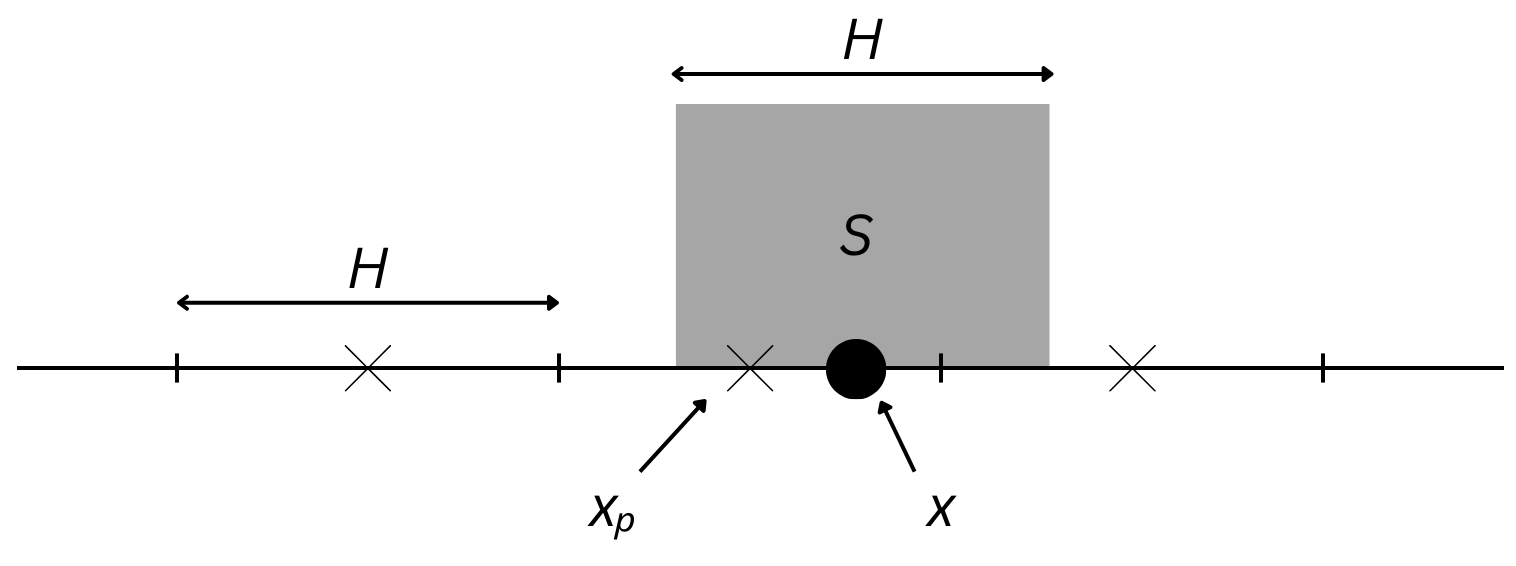
\includegraphics[scale=0.2]{chapters/pm-method/img/CIC.png}
    \caption{The CIC shape centered at $x$ (particle position).
        The particle is within cell $x_p$; however, the cell $x_{p+1}$ gets a non-zero density contribution from the particle.}
    \label{fig:cic-shape}
\end{figure}

In the one-dimensional case, the fraction of mass $W_p$ assigned to mesh-point $p$ from particle at position $x$ is given by
\begin{equation*}
    W(x-x_p) = W_p(x) = \int_{x_p-H/2}^{x_p+H/2} dx' S(x'-x).
\end{equation*}
A simple rule for relating the assignment function $W$ defined above with shape $S$ can be found by noticing that
\begin{equation*}
    W(x) = \int_{-H/2}^{H/2}dx' S(x'-x) = \int_{-\infty}^\infty dx' \Pi\left(\frac{x'}{H}\right)S(x'-x) = \Pi\left(\frac{x}{H}\right) * S(x).
\end{equation*}
This implies that
\begin{align}\label{eq:assignment-functions}
    W_\text{NGP}(x) & = \Pi\left(\frac{x}{H}\right), & W_\text{CIC}(x) & = \Lambda\left(\frac{x}{H}\right), & W_\text{TSC}(x) & = \Pi\left(\frac{x}{H}\right) * \frac{1}{H} \Lambda\left(\frac{x}{H}\right) = (\Pi * \Lambda)\left(\frac{x}{H}\right).
\end{align}
Splitting the domain of integration in the expression for $W_\text{TSC}$ into five disjoint intervals shows that
\begin{equation*}
    (\Pi * \Lambda)(x) = \begin{cases}
        \frac{1}{8}(3-2|x|)^2, & \frac{1}{2} \leq |x| < \frac{3}{2} \\
        \frac{3}{4}-x^2,       & |x| < \frac{1}{2}                  \\
        0,                     & \text{otherwise}.
    \end{cases}
\end{equation*}

Two- and three-dimensional versions of the assignment functions in \autoref{eq:assignment-functions} are products of the assignment functions in each dimension.
For example, the three-dimensional assignment function $W$ is
\begin{equation*}
    W(\mathbf{x}) = W(x)W(y)W(z).
\end{equation*}
Hence, the mass assigned at mesh-point at $\mathbf{x}_\mathbf{p}$ is
\begin{equation*}
    m(\mathbf{x}_\mathbf{p}) = \sum_i m_i W_\mathbf{p}(\mathbf{x}_i),
\end{equation*}
or, in terms of density $\rho$,
\begin{equation}\label{eq:density-assignment}
    \rho(\mathbf{x}_\mathbf{p}) = \frac{1}{V} \sum_i m_i W_\mathbf{p}(\mathbf{x}_i),
\end{equation}
where $V = H^3$ is the volume of a cell and $i$ indexes the particles.

Obviously, \autoref{eq:density-assignment} is not suitable for direct application in the actual algorithm.
Instead, we iterate over all particles, identify the parent cell $\mathbf{p}$ of each particle (and the neighborhood of $\mathbf{p}$) and update $\rho$.
This process is illustrated in \autoref{alg:density-assignment}.
\begin{algorithm}
    \caption{Density assignment algorithm}\label{alg:density-assignment}
    \begin{algorithmic}[1]
        \ForAll {particle $i$}
        \ForAll {cell $\mathbf{q}$ in $\mathcal{C}_S(\mathbf{x}_i)$}
        \State $\rho(\mathbf{x}_\mathbf{q}) \gets \rho(\mathbf{x}_\mathbf{q}) + m_i W(\mathbf{x}_i - \mathbf{x}_\mathbf{q}) / V$
        \EndFor
        \EndFor
    \end{algorithmic}
\end{algorithm}
The set $\mathcal{C}_S(\mathbf{x}_i)$ of cells that have to be considered while assigning density from the $i$-th particle depends on the shape $S$ of the particle.
Specifically, we have $\mathcal{C}_\mathrm{NGP}(\mathbf{x}) = \{[\mathbf{x} / H]\}$, $\mathcal{C}_\mathrm{CIC}(\mathbf{x}) = \{\lfloor \mathbf{x}/H \rfloor + \mathbf{t} \;|\; t_i =0,1\}$, and $\mathcal{C}_\mathrm{TSC}(\mathbf{x}) = \{[\mathbf{x} / H] + \mathbf{t} \;|\; t_i = -1, 0, 1\}$.
It follows that $|\mathcal{C}_\mathrm{NGP}(\mathbf{x})| = 1$, $|\mathcal{C}_\mathrm{CIC}(\mathbf{x})| = 8$, and $|\mathcal{C}_\mathrm{TSC}(\mathbf{x})| = 27$ which illustrates the increasing computational cost resulting from using higher-order assignment schemes.
We note that \autoref{alg:density-assignment} is easily parallelized if atomic increments are used in line 3.

\section{Solving the field equation}\label{sec:solving-the-field-equation}
The Poisson equation (\autoref{eq:poisson}) can be restated in integral form
\begin{equation*}
    \phi(\mathbf{x}) = \int d\mathbf{x}' \mathcal{G}(\mathbf{x}-\mathbf{x}')\rho(\mathbf{x}'),
\end{equation*}
which has the following discrete analogue
\begin{equation}\label{eq:poisson-discrete}
    \phi(\mathbf{x}_\mathbf{p}) = V \sum_{\mathbf{p}'} \mathcal{G}(\mathbf{x}_\mathbf{p} - \mathbf{x}_{\mathbf{p}'}) \rho(\mathbf{x}_{\mathbf{p}'}),
\end{equation}
where $\mathcal{G}$ is the Green's function (potential due to unit mass).
The right-hand side of \autoref{eq:poisson-discrete} is a convolution sum over a finite set of mesh points.
If we assume periodic boundary conditions, we can apply the discrete Fourier transform to both sides and use the convolution theorem to conclude that\footnote{
    In this work, the Hockney \& Eastwood definition of DFT is used, i.e.,
    \begin{equation*}
        D(x_p) = \frac{1}{L}\sum_{l=0}^{N-1}\hat{D}(k)e^{ikx_p}, \quad \hat{D}(k) = H\sum_{p=0}^{N-1}D(x_p)e^{-ikx_p},
    \end{equation*}
    where $x_p = pH$ and $k=2\pi l / L$ ($L$ is the mesh period length equal to $NH$).
    The three-dimensional transform is obtained by replacing $x \to \mathbf{x}=(x_1, x_2, x_3)$, $k \to \mathbf{k}=(k_1, k_2, k_3)$, $kx \to \mathbf{k} \cdot \mathbf{x}$, $L \to L_1 L_2 L_3$, $H \to H_1 H_2 H_3$, and so on.
}
\begin{equation}\label{eq:poisson-fourier-product}
    \hat{\phi}(\mathbf{k}) = \hat{\mathcal{G}}(\mathbf{k}) \hat{\rho}(\mathbf{k}).
\end{equation}

An approximation to $\hat{\mathcal{G}}$ can be found using a discretized version of the Laplacian in \autoref{eq:poisson}.
Specifically, for a 7-point stencil,
\begin{equation*}
    \begin{split}
        4\pi G\rho(\mathbf{x}_{ijk})
         & =\frac{\phi(\mathbf{x}_{i-1,j,k}) - 2\phi(\mathbf{x}_{ijk})+\phi(\mathbf{x}_{i+1,j,k})}{H^2}   \\
         & + \frac{\phi(\mathbf{x}_{i,j-1,k}) - 2\phi(\mathbf{x}_{ijk})+\phi(\mathbf{x}_{i,j+1,k})}{H^2}  \\
         & + \frac{\phi(\mathbf{x}_{i,j,k-1}) - 2\phi(\mathbf{x}_{ijk})+\phi(\mathbf{x}_{i,j,k+1})}{H^2}.
    \end{split}.
\end{equation*}
Applying the discrete Fourier transform to both sides and using the shift theorem, we get
\begin{align*}
    4\pi G \hat{\rho}(\mathbf{k})
     & = \frac{1}{H^2}\sum_{i=1}^{3}\left( e^{-iHk_i} + e^{iHk_i}-2 \right)\hat{\phi}(\mathbf{k})       \\
     & = \frac{1}{H^2} \sum_{i=1}^{3}\left( e^{iHk_i/2} - e^{-iHk_i/2} \right)^2 \hat{\phi}(\mathbf{k}) \\
     & = -\frac{4}{H^2}\sum_{i=1}^{3}\sin^2\left(\frac{Hk_i}{2}\right)\hat{\phi}(\mathbf{k}).
\end{align*}
and hence
\begin{equation}\label{eq:dft-transformed-phi}
    \hat{\phi}(\mathbf{k}) = -4\pi G\underbrace{\frac{(H/2)^2}{\sin^2(Hk_1/2) + \sin^2(Hk_2/2) + \sin^2 (Hk_3/2)}}_{\hat{\mathcal{G}}(\mathbf{k})} \hat{\rho}(\mathbf{k}),
\end{equation}
where $\hat{\mathcal{G}}$ can be identified by comparison with \autoref{eq:poisson-fourier-product}.
It is worth noting that the constant multiplier $(-4\pi G)$ is often left out of $\hat{\mathcal{G}}$ (this is the convention used in \cite{Hockney1988}).
In the implementation, values of $\hat{\mathcal{G}}$ are computed only once and saved for future look-up.

In the one-dimensional case, the above discussion can be easily rephrased in terms of a diagonalization problem \cite{demanet2013fourier}.
In one dimension, the Poisson equation is
\begin{equation}\label{eq:poisson-1d}
    \Delta \phi \equiv \frac{d^2 \phi}{dx^2} = \rho.
\end{equation}
The interval $[a, b]$ (of length $L = b-a$) on which we wish to find $\phi$ is assumed to be discretized into $N$ points $x_j = a + H/2 + jH$, where $H = L / N$ and $j=0,\dots, N-1$.
Furthermore, we assume periodic boundary conditions so that $\phi(x_{-1}) = \phi(x_{N-1})$ and $\phi(x_{N}) = \phi(x_0)$.
The approximation of $\Delta$ at $x_j$ is
\begin{equation*}
    (\Delta_H \phi)_j \equiv -\frac{\phi_{j-1} - 2\phi_j + \phi_{j+1}}{H^2}.
\end{equation*}
Thus, the discrete version of \autoref{eq:poisson-1d} reads $-(\Delta_H \phi)_j = \rho_j$ or
\begin{equation*}
    \frac{\phi_{j-1}-2\phi_j + \phi_{j+1}}{H^2} = \rho_j,
\end{equation*}
where $\rho_j = \rho(x_j)$.
This gives us a system of $N$ equations (one per each sampled value of $\rho$) with $N$ unknowns (values of $\phi$) of the following form
\begin{equation}\label{eq:poisson-1d-matrix}
    -\underbrace{\frac{1}{H^2}
        \begin{bmatrix}
            2  & -1     &        &        & -1 \\
            -1 & 2      & \ddots &        &    \\
               & \ddots & \ddots & \ddots &    \\
               &        & \ddots & 2      & -1 \\
            -1 &        &        & -1     & 2
        \end{bmatrix}}_{\Delta_H}
    \underbrace{\begin{bmatrix}
            \phi_0     \\
            \phi_1     \\
            \vdots     \\
            \phi_{N-2} \\
            \phi_{N-1}
        \end{bmatrix}}_{\bar{\phi}}
    = \underbrace{\begin{bmatrix}
            \rho_0     \\
            \rho_1     \\
            \vdots     \\
            \rho_{N-2} \\
            \rho_{N-1}
        \end{bmatrix}}_{\bar{\rho}}.
\end{equation}
Next we define $\bar{\psi}(l) \in \mathbb{C}^N$ by $\psi_j(l) \equiv e^{i2\pi jl/N} = \omega^{jl}$ for $j=0,\dots,N-1$.
The $j$-th row of $H^2\Delta_H \bar{\psi}$ equals
\begin{align*}
    (H^2\Delta_H \bar{\psi})_j
     & = -\psi_{j-1} + 2\psi_j - \psi_{j+1}
    = -\omega^{(j-1)l} + 2\omega^{jl} - \omega^{(j+1)l}     \\
     & = -\omega^{jl}(\omega^{-l} - 2 + \omega^l)
    = -\omega^{jl}(\omega^{l/2} - \omega^{-l/2})^2          \\
     & = 4\omega^{jl} \sin^2\left( \frac{\pi l}{N} \right).
\end{align*}
Hence we have $(H^2\Delta_H \bar{\psi})_j = 4\sin^2(\pi l/N) \psi_j$ which implies
\begin{equation*}
    \Delta_H \bar{\psi}(l)
    = \frac{4}{H^2} \sin^2\left( \frac{\pi l}{N} \right) \bar{\psi}(l).
\end{equation*}
This result tells us that for any value of $l$, $\bar{\psi}(l)$ is an eigenvector of $\Delta_H$ with eigenvalue $(4/H^2)\sin^2(\pi l/N)$.
For $l=0,\dots, N-1$ we get $N$ linearly independent eigenvectors $\{\bar{\psi}(l)\}$ which necessarily form the basis of $\mathbb{C}^N$.
This fact implies that $\Delta_H$ is diagonalizable.
The matrix $F$ of its eigenvectors is given by $F_{jl} = (1/L) \omega^{jl}$, and the inverse is easily verified to be $F^{-1} = LH F^\dagger$, where the dagger denotes Hermitian adjoint.
The eigendecomposition of $\Delta_H$ is therefore
\begin{equation*}
    \Delta_H = F\Lambda F^{-1},
\end{equation*}
where $\Lambda = \text{diag}((4/H^2)\sin^2(\pi l/N))$.
Substitution into \autoref{eq:poisson-1d-matrix} yields $F\Lambda F^{-1} \bar{\phi} = -\bar{\rho}$ or
\begin{equation*}
    F^{-1}\bar{\phi} = -\Lambda^{-1}F^{-1}\bar{\rho}.
\end{equation*}
Evaluating the left-hand side leads to the conclusion that $F^{-1}\bar\phi$ is nothing but the DFT of $\bar\phi$.
Indeed,
\begin{equation*}
    (F^{-1}\phi)_j
    = LH (F^\dagger \phi)_j
    = LH \sum_{l=0}^{N-1}F^\dagger_{jl}\phi_l
    = H \sum_{l=0}^{N-1}\omega^{-lj}\phi_l
    = H \sum_{l=0}^{N-1}e^{-i2\pi jl / N}\phi_l
\end{equation*}
which is precisely the discrete Fourier transform of $\bar\phi$.
Thus, we see that the DFT of the Green's function, $\hat{\mathcal{G}}(k) = \hat{\mathcal{G}}(2\pi l / L)$, derived in \autoref{eq:dft-transformed-phi}, is the reciprocal of the $l$-th eigenvalue of the discretized Laplacian $(-\Delta_H)$.
Following the line of reasoning presented above, we observe a deep connection between the DFT and the eigendecomposition of the discretized Laplace operator.

A natural question that arises in the context of this discussion is whether a similar relation holds in the continuous case.
The answer turns out to be positive;
assuming free-space boundary conditions, the complex exponential $e^{i \mathbf{k} \cdot \mathbf{x}}$ (kernel of the inverse Fourier transform) is an eigenfunction of the Laplace operator (with eigenvalue $-k^2$) and the Fourier transform allows for a diagonalization of the Laplacian \cite{demanet2013fourier}.
More precisely, we have
\begin{equation*}
    \Delta = F \Lambda F^{-1},
\end{equation*}
where $F$ is the inverse FT, and $\Lambda = -k^2$.
Applying this result to the Poisson equation yields $F^{-1}\phi = \Lambda^{-1}F^{-1}\rho$ or
\begin{equation}\label{eq:poor-mans-poisson-solver}
    \hat\phi = -\frac{1}{k^2} \hat\rho,
\end{equation}
where the circumflex denotes the Fourier transform and $k = |\mathbf{k}|$.
The function $(-1/k^2)$ is sometimes used instead of the transformed Green's function $\hat{\mathcal{G}}$ defined in \autoref{eq:dft-transformed-phi}.
This approach is the basis of the ``poor man's Poisson solver'' (as dubbed by \cite{Hockney1988}).
While implementing it, we have to take into account that in the standard definition of the DFT, nonnegative frequencies correspond to $0 \leq l \leq N/2$ and negative frequencies correspond to $N/2+1 \leq l \leq N-1$ (see \cite{press2007numerical}, pp. 607--608).
This necessitates the following ``index wrapping'':
\begin{equation*}
    l_i =
    \begin{cases}
        i     & \text{if } i \leq \frac{N}{2} \\
        i - N & \text{if } i > \frac{N}{2}
    \end{cases},
\end{equation*}
where $i$ is the index of the gridpoint.

\section{Field strength calculation}
The strength $\mathbf{g}$ of the gravitational field at mesh point $\mathbf{x}_\mathbf{p}$ can be approximated using a central finite difference.
Our implementation supports two types of finite differences, defined below as two variants of a particular operator.
\begin{enumerate}
    \item The $j$-th component ($j = x, y, z$) of the two-point finite difference operator $\mathbf{D}$ is given by
          \begin{equation}\label{eq:two-point-central-diff-def-1}
              D_j(\phi)(\mathbf{x}_\mathbf{p}) = \frac{\phi(\mathbf{x}_{p} + H\mathbf{e}_j) - \phi(\mathbf{x}_\mathbf{p} - H\mathbf{e}_j)}{2H},
          \end{equation}
          where $\mathbf{e}_j$ is the $j$-th standard basis vector.
          This scheme is second-order accurate.
    \item The four-point finite difference operator $\mathbf{D}$ is defined in terms of its components $j$ as
          \begin{equation*}
              D_j(\phi)(\mathbf{x}_\mathbf{p}) = \alpha\frac{\phi(\mathbf{x}_{p} + H\mathbf{e}_j) - \phi(\mathbf{x}_\mathbf{p} - H\mathbf{e}_j)}{2H} + (1-\alpha)\frac{\phi(\mathbf{x}_\mathbf{p} + 2H\mathbf{e}_j) - \phi(\mathbf{x}_\mathbf{p} - 2H\mathbf{e}_j)}{4H}.
          \end{equation*}
          The scheme is fourth-order accurate for $\alpha = 4/3$.
\end{enumerate}

The difference between the accuracy of both methods is illustrated in \autoref{fig:finite-diff-accuracy}.
The figure also provides insight into how the error depends on the value of parameter $\alpha$.
\begin{figure}[htp]
    \centering
    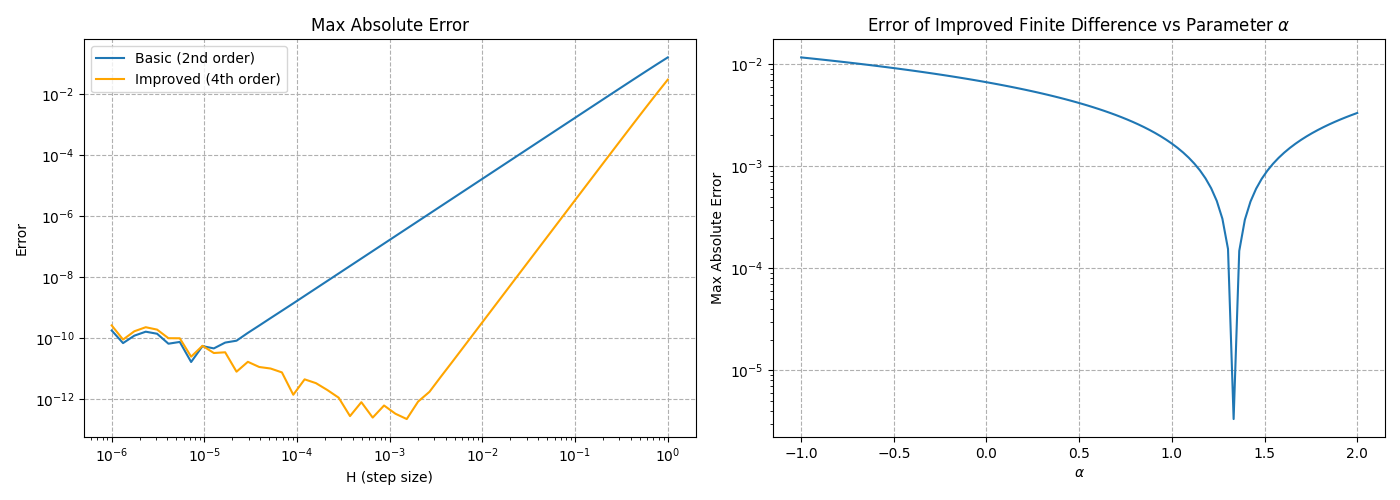
\includegraphics[scale=0.43]{chapters/pm-method/img/finite-difference.png}
    \caption{Left panel: Approximation error for second-order and fourth-order schemes.
        For small values of $H$, round-off errors dominate.
        Right panel: Approximation error vs. $\alpha$ in the improved finite difference scheme ($H = 0.1$).
        Note that the scheme is fourth-order accurate only for $\alpha = 4/3$ (cusp in the graph).}
    \label{fig:finite-diff-accuracy}
\end{figure}

We can alternatively define the finite differences in terms of the delta function to get rid of the dependence on the differenced function. (Technically, the resulting quantities are functions rather than operators.)
Consider, for example, the two-point finite difference in \autoref{eq:two-point-central-diff-def-1} and notice that
\begin{equation*}
    D_j(\phi)(\mathbf{x}) = \frac{\phi(\mathbf{x} + H \mathbf{e}_j)-\phi (\mathbf{x} - H \mathbf{e}_j)}{2H} = \int d\mathbf{x}' \left[ \frac{\delta(\mathbf{x} + H\mathbf{e}_j - \mathbf{x}') - \delta(\mathbf{x} - H\mathbf{e}_j - \mathbf{x}')}{2H} \right]\phi(\mathbf{x}').
\end{equation*}
Thus, we see that
\begin{equation}\label{eq:two-point-central-diff}
    D_j(\mathbf{x}) = \frac{\delta(\mathbf{x} + H\mathbf{e}_j) - \delta(\mathbf{x} - H\mathbf{e}_j)}{2H}
\end{equation}
and
\begin{equation}\label{eq:four-point-central-diff}
    D_j(\mathbf{x}) = \alpha\frac{\delta(\mathbf{x} + H\mathbf{e}_j) - \delta(\mathbf{x} - H\mathbf{e}_j)}{2H} + (1-\alpha)\frac{\delta(\mathbf{x} + 2H\mathbf{e}_j) - \delta(\mathbf{x} - 2H\mathbf{e}_j)}{4H}
\end{equation}
are directly related to the kernels of the two-point and four-point finite difference operators, respectively.
In symbols,
\begin{equation*}
    \mathbf{D}(\phi)(\mathbf{x}) = \int d\mathbf{x}' \mathbf{D}(\mathbf{x} - \mathbf{x}')\phi(\mathbf{x}').
\end{equation*}

If $\phi$ denotes the gravitational potential, then the field $\mathbf{g}$ is approximated at mesh point $\mathbf{x}_\mathbf{p}$ as
\begin{equation*}
    \mathbf{g}(\mathbf{x}_\mathbf{p}) = -\mathbf{D}(\phi)(\mathbf{x}_\mathbf{p}),
\end{equation*}
which is the discrete version of the relation $\mathbf{g} = -\nabla \phi$.

\section{Interpolation}
The value of the field strength $\mathbf{g}(\mathbf{x})$ at the position particle's position $\mathbf{x}$ is calculated by interpolating the values of $\mathbf{g}$ from the neighboring mesh-points.
Formally,
\begin{equation*}
    \mathbf{g}(\mathbf{x}) = \sum_\mathbf{p} W(\mathbf{x} - \mathbf{x}_\mathbf{p}) \mathbf{g}(\mathbf{x}_\mathbf{p}).
\end{equation*}
In practice, there is no need to sum over all mesh points.
Instead, we use an algorithm analogous to \autoref{alg:density-assignment} to only include the cells with non-zero contribution to the sum.
The method is illustrated in \autoref{alg:interpolation}.
\begin{algorithm}
    \caption{Field strength interpolation}\label{alg:interpolation}
    \begin{algorithmic}[1]
        \ForAll {particle $i$}
        \ForAll {cell $\mathbf{q}$ in $\mathcal{C}_S(\mathbf{x}_i)$}
        \State $\mathbf{g}(\mathbf{x}_i) \gets \sum_\mathbf{q} W(\mathbf{x}_i - \mathbf{x}_\mathbf{q}) \mathbf{g}(\mathbf{x}_\mathbf{q})$
        \EndFor
        \EndFor
    \end{algorithmic}
\end{algorithm}
It is important to note that in order to retain correct physical behavior, the interpolation and mass assignment schemes must use the same shape to represent the particles.
The procedure in \autoref{alg:interpolation} is trivially parallelized by converting the sequential loop into a parallel one.

The procedures of density assignment and interpolation presented in \autoref{alg:density-assignment} and \autoref{alg:interpolation} are high level description.
More concrete formulations suitable for direct use in an implementation are given in \cite{Hockney1988} and \cite{Kravtsov2002PM}.

\section{Code units}
Implementation of the PM (and \PThreeM{}) methods can be simplified by switching to a system of dimensionless units, often called \textit{code units}.
The natural units of time and length in a PM simulation are $H$ and $DT$, respectively.
Hence, length in a PM code is conveniently expressed in terms of multiples of $H$, and similarly, time intervals are given as a multiple of $DT$, i.e., the conversion relations are
\begin{equation*}
    x' = \frac{x}{H} \quad \text{and} \quad t' = \frac{t}{DT}.
\end{equation*}
From there, it follows that
\begin{equation*}
    v' = \frac{DT}{H}v \quad \text{and} \quad a' = \frac{DT^2}{H}a.
\end{equation*}
The expected relation $\mathbf{g}' = -\nabla' \phi'$ leads to the definition $\phi' = (DT^2 / H^2)\phi$.
By stipulating that we have $\nabla'^2\phi = \rho'$, we get $\rho' = DT^2 \cdot 4\pi G\rho$, $m' = (DT^2\cdot 4\pi G / H^3) m$, and $G' = 1/(4\pi)$.

\section{Properties of the calculated field}
The accuracy of a simulation using a PM code depends on several factors.
The user can decide to use any combination of the following elements that parameterize the program:
\begin{itemize}
    \item mass assignment and interpolation scheme: NGP, CIC, TSC, or possibly any other scheme from the infinite hierarchy described in \autoref{sec:mass-assignment};
    \item convolution with the Green's function derived from the discretized Laplacian (\autoref{eq:dft-transformed-phi}) or the ``poor man's solver'' (\autoref{eq:poor-mans-poisson-solver});
    \item gradient approximation: two-point or four-point finite difference;
    \item grid resolution: number of meshpoints in each dimension.
\end{itemize}
In this subsection, we analyze these choices from two different angles.
We first focus on the properties of the field produced by a single source, which provides insight into the behavior of the simulation based on pairwise interparticle interactions.
Then, we analyze the global error in force calculation by comparing the PM-calculated forces acting on all particles in a typical simulation with forces produced by the PP method.

\subsection{Local picture}
The field produced by the PM method is neither homogenous nor isotropic.
Anisotropy can be observed by measuring the field generated by a particle in two different directions.
In \autoref{fig:pm-field-properties}, the field strength calculated using the PM method (with the Green's function derived from discrete Laplacian) due to a single source at $x = H$ is shown in two variants: when measured along the $x$-axis (blue line) and the $x=y$ line (orange line).
The difference between these two graphs illustrates the anisotropy of the calculated field.
The figure also shows the field strength measured along the $x$-axis when the source was shifted by $H/2$ in the $-x$ direction (green line).
Its deviation from the case when the source was placed at $x=H$ (the blue graph) exemplifies the inhomogeneity of the field computed using the PM method.
\begin{figure}[!ht]
    \centering
    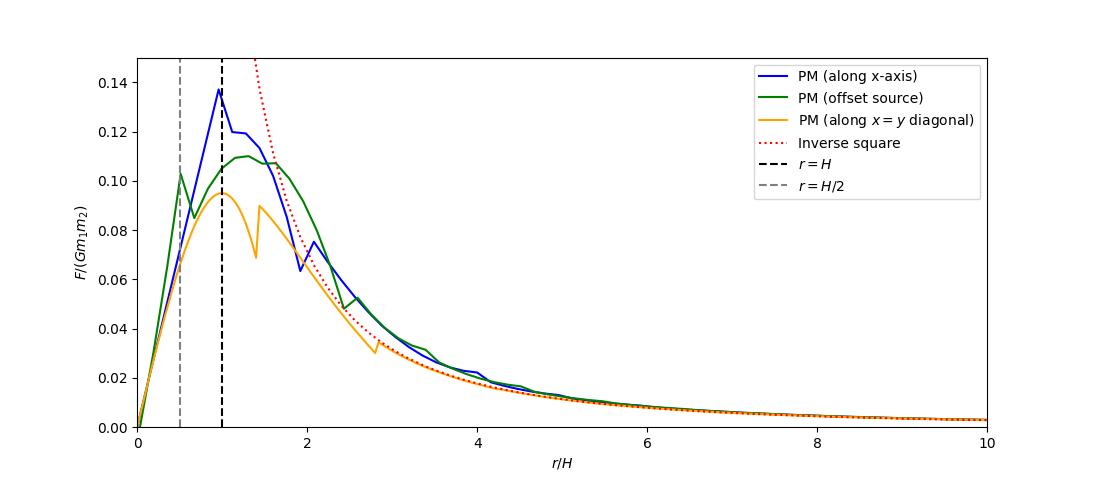
\includegraphics[scale=0.55]{chapters/pm-method/img/pm-field-combined.png}
    \caption{Anisotropy and inhomogeneity of the field as calculated by the PM method (TSC assignment, second-order finite difference).}
    \label{fig:pm-field-properties}
\end{figure}
As expected, the PM-calculated approximation gets better with increasing distance from the source;
the inverse-square law is reproduced accurately for $r \gtrsim 4H$.

The single-source case analysis can be extended by considering the effect of choice of finite difference and mass assignment schemes on the relative error between the actual and approximated field strength.
\autoref{fig:pm-combined} shows a comparison of (a) the relative error as a function of distance from the source for PM with second-order and fourth-order finite differences and (b) the field strength computed using different mass assignment schemes discussed in \autoref{sec:mass-assignment}.
\begin{figure}[!ht]
    \centering
    \begin{subfigure}[t]{0.48\textwidth}
        \centering
        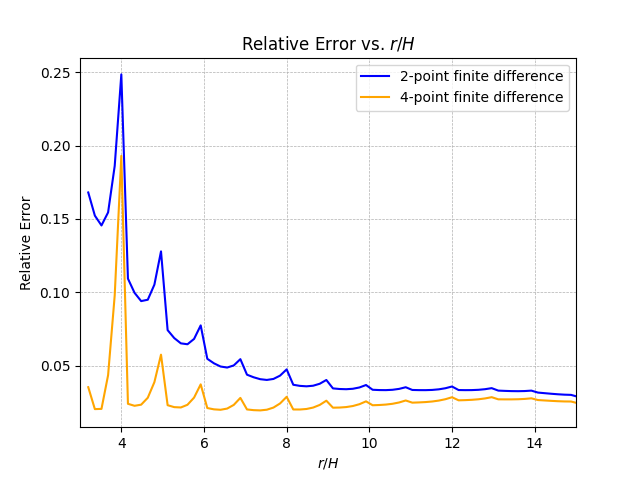
\includegraphics[width=\linewidth]{chapters/pm-method/img/pm-finite-diff-err.png}
        \caption{Relative error of field strength approximation in different finite difference schemes.}
        \label{fig:pm-finite-diff-err}
    \end{subfigure}
    \hfill
    \begin{subfigure}[t]{0.48\textwidth}
        \centering
        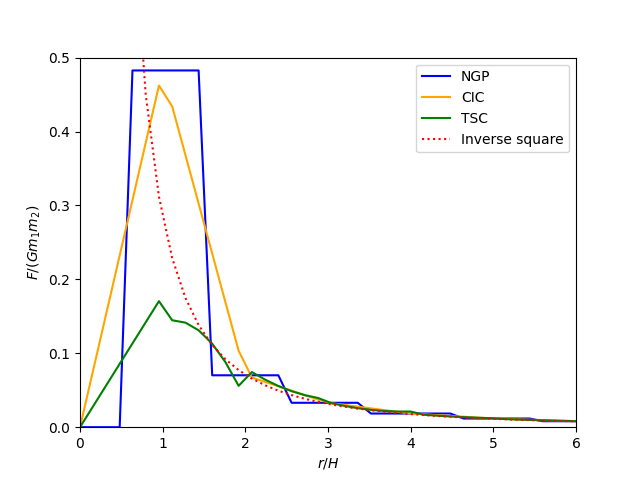
\includegraphics[width=\linewidth]{chapters/pm-method/img/pm-mass-assignment.png}
        \caption{Field strength calculated with the PM method using different assignment schemes (four-point finite difference).}
        \label{fig:pm-mass-assignment-field-strength}
    \end{subfigure}
    \caption{Approximation quality in the PM method.}
    \label{fig:pm-combined}
\end{figure}
The conclusion that can be drawn from \autoref{fig:pm-combined} is that, as expected, the TSC mass assignment scheme and the four-point finite difference yield the best results.

The field produced by the PM method using the ``poor man's'' potential solver is similar to the one obtained using the discretized Laplacian Green's function described above (see \autoref{fig:pm-poor-man-vs-laplacian}).
\begin{figure}[!ht]
    \centering
    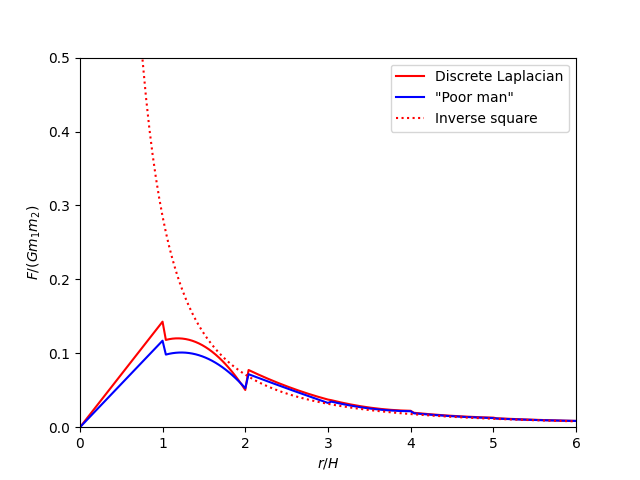
\includegraphics[scale=0.55]{chapters/pm-method/img/poor-man-vs-laplacian.png}
    \caption{Field obtained potential calculated by the ``Poor man's Poisson solver'' vs. when using \autoref{eq:dft-transformed-phi}.}
    \label{fig:pm-poor-man-vs-laplacian}
\end{figure}

\subsection{Global picture}\label{subsubsec:pm-global-picture}
To calculate the global approximation error of a PM simulation, we calculated the average of relative differences over all particles ($N=10{,}000$ in this case) between the forces produced by the PM method and the exact result obtained using the PP method.
More precisely, the error was defined as
\begin{equation}\label{eq:force-avg-relative-err}
    \frac{1}{N}\sum_{i} \frac{|\mathbf{F}_i^\text{approx.} - \mathbf{F}_i^\text{PP}|}{|\mathbf{F}_i^\text{PP}|}.
\end{equation}
The result for different grid resolutions is shown in \autoref{fig:pm-global-err-lap} ( $30 \leq N_g \leq 70$).
For this test, the particle positions were generated according to the uniformly decreasing density disk model.
\begin{figure}[!ht]
    \centering
    \begin{subfigure}[t]{0.48\textwidth}
        \centering
        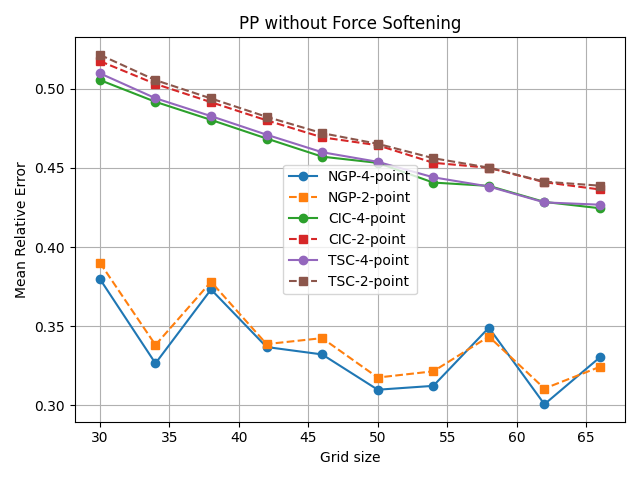
\includegraphics[width=\linewidth]{chapters/pm-method/img/pm-global-err.png}
        \caption{PP calculation without force softening.}
        \label{fig:pm-global-err-lap-no-soft}
    \end{subfigure}
    \hfill
    \begin{subfigure}[t]{0.48\textwidth}
        \centering
        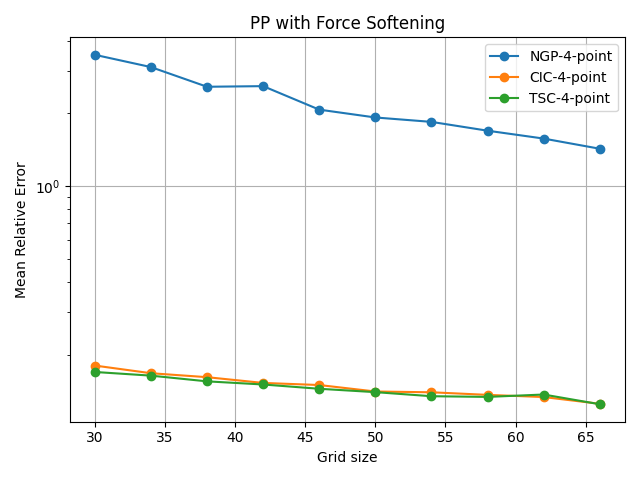
\includegraphics[width=\linewidth]{chapters/pm-method/img/pm-global-err-soft.png}
        \caption{PP calculation with force softening.}
        \label{fig:pm-global-err-lap-soft}
    \end{subfigure}
    \caption{Average force approximation error in the PM method (discrete Laplacian solver).}
    \label{fig:pm-global-err-lap}
\end{figure}
As can be seen in \autoref{fig:pm-global-err-lap-no-soft}, for each of the assignment schemes, the error is minimized for the four-point difference, as expected;
a more surprising result is that the errors are most significant for the TSC assignment scheme.
This paradox is easily explained by considering the graphs in \autoref{fig:pm-mass-assignment-field-strength}.
As can be seen there, the TSC assignment scheme gives rise to a force that accurately reproduces the inverse-square law force, but at the same time, it severely underestimates the force close to the source.
This behavior is expected since it stems from the mass of any individual particle being spread between multiple cells.
The CIC and NGP schemes, on the other hand, do not reproduce the actual force with the same level of accuracy, but the underestimation close to the source is not as severe as in the case of the TSC scheme.
In some applications, for instance, in the context of a galaxy simulation, this is a favorable feature of the TSC scheme.
The number of stars in a galaxy can be in the order of $10^{12}$ \cite{young2006andromeda}, whereas the number of particles in our tests is in the order of tens of thousands, giving an average of around $10^{12} / 10^{4} = 10^8$ of stars per particle.
Hence, it would be a grave mistake to model the force due to a single particle by the force due to a dimensionless point mass.
In such a case, it is a standard practice to use a softened gravitational force instead of the one given in \autoref{eq:law-of-uni-grav} \cite{10.1046/j.1365-8711.2000.03316.x}.
By using the TSC scheme, force softening is automatically included in the calculation.
It can be argued that obtaining the smoothness properties enjoyed by the higher-order assignment schemes should be treated as tangential to softening the force.
It is for this reason that Hockney and Eastwood introduce the notion of \textit{force sharpening} as an additional step in the PM method in \cite{Hockney1988}.
In this modified version of the PM method, the Poisson equation takes the form
\begin{equation*}
    \nabla^2 \phi_p = \rho_p^*,
\end{equation*}
where $\rho^*_p$ is obtained from the density $\rho_p$ by solving the following system
\begin{equation*}
    1+\frac{\rho^*_{p+1} - 2\rho^*_p + \rho^*_{p-1}}{8}
    = \rho_p,
\end{equation*}
where $p$ indexes the mesh points.
In this work, we do not investigate this matter further, nor do we implement this modification in our program.

Now we return to the test whose results are presented in \autoref{fig:pm-global-err-lap}.
In the light of the above discussion, it is more reasonable to compare the quality of the results of the PM method with a \textit{softened gravitational force} defined in \cite{Zhang_2019} as
\begin{equation}\label{eq:softened-force}
    \mathbf{F}^\textrm{soft}_{ij} = -G\frac{m_i m_j}{(r_{ij}^2 + \epsilon^2)^{3/2}}\mathbf{r}_{ij}.
\end{equation}
The relative difference between the softened forces and the PM-calculated ones is shown in \autoref{fig:pm-global-err-lap-soft}.
The \textit{softening length} in the PP method was set at $\epsilon = H$ in each run of the test so that it roughly matches the softening ``induced'' by the PM method (cf. \autoref{fig:pm-mass-assignment-field-strength}).

\section{Implementation}
\subsection{CPU variant}
The most computationally involved step of the PM method is the happens in the potential solver.
As explained in \autoref{subsec:solving-the-field-equation}, in our implementation we solve the Poisson equation for the potential using the convolution method.
This involves taking the DFT of the grid-defined density and later the inverse DFT of the product of transformed Green's function and the transformed density.
Since the number of grid points in a typical grid can be of the order of a million, choosing the right implementation of the FFT is of paramount importance.
We tried incorporating a handful of popular C++ FFT libraries into the program and out of those considered, FFTW (\url{https://www.fftw.org/}) and kissfft (\url{https://github.com/mborgerding/kissfft}) provided best performance.
The running times for FFT and inverse FFT stages of the algorithm using each of the libraries are shown in \autoref{fig:cic-shape}.
\begin{figure}[htp]
    \centering
    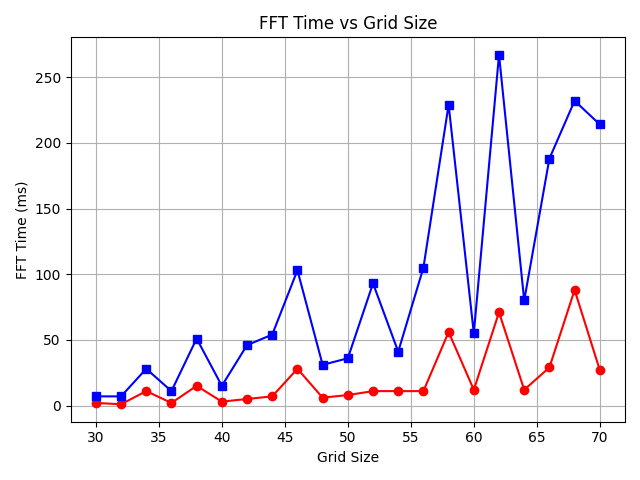
\includegraphics[scale=0.5]{img/fft_time.png}
    \caption{Time needed to perform the DFT and inverse DFT using kissft and FFTW libraries.
        The total grid size in the test was $(2N_g)\times (2N_g) \times N_g$, where $N_g$ is labeled as ``Grid Size'' on the horizontal axis in the graph.}
    \label{fig:fft-time}
\end{figure}
As we can see, FFTW considerably outperformed kissfft, with the former achieving an average five-fold speedup over the latter.
Interestingly, most spikes in the running time, taking place for certain grid sizes

As noted in \autoref{subsec:mass-assignment}, parallelization of the mass assignment step which involves ``spreading'' the mass due to a particle over nearby cells, requires synchronization to avoid data races.
The above requirement can be fulfilled by using mutexes or atomic operations.
Traditionally, atomic RMW operations were supported by the C++ standard library only for the integer types, however recently C++20 introduced atomic RMW operations on floating point numbers (see \url{https://en.cppreference.com/w/cpp/atomic/atomic.html}).
We conducted a simple benchmark on Intel Core i7-9750H CPU (three threads concurrently incrementing a global variable) to compare the performance of both approaches.
The benchmark indicated that guarding the critical section with a mutex was around two times faster than using atomic operations.
However, the same test run on a system with a different processor indicated that using atomic counter offers better performance, which shows that more careful benchmarking would be needed to reach a definite conclusion.

\subsection{GPU variant}
As explained before, the mass assignment, field calculation at mesh points, and interpolation steps of the PM method are embarrassingly parallel.
For this reason rewriting the PM code for the GPU does not pose much difficulty.
In our implementation we used CUDA C++ language extension to implement the method on the GPU.
A thorough introduction to the arcana of programming NVIDIA GPU devices is given in \cite{nvidia2025cuda}.
In this work, we only remark on the aspects directly related to our use case.

The memory hierarchy of a GPU (also referred to as the \textit{device}) is organized into three main levels:
\begin{enumerate}
    \item global memory (accessible by all threads as well as \textit{host} (CPU); high latency),
    \item shared memory (accessible by threads in the same threadblock typically up to 48 KB; very low latency),
    \item local storage (per thread storage in the form of registers managed by the compiler).
\end{enumerate}
We recognized that one step of the PM method that could potentially benefit from transferring data to shared memory is the gradient calculation step.
For example, if the 2-point finite difference approximation to the Laplacian is used, the potential from six cells needs to be fetched from memory.
At the same time, there is an overlap between the potential data read by threads working on adjacent mesh cells.
Thus, theoretically, fetching the potential data into shared memory could have positive impact on performance.
However, our tests for the 2-point approximation, performed at early stages of the development of the program did not indicate significant improvement in the running time of the algorithm and this optimization path was not explored further.

A major performance bottleneck in the GPU implementation is transferring the data between host and device.
These data transfers are necessary if one wishes to record the state of the simulation after each timestep.
If only the final state of the simulation is of interest, then the PM method can execute entirely on the device transferring the data to the host only once after the final iteration of the simulation.
This is the scenario that we assumed for the purpose of comparing the CPU and GPU implementation.
The results of the test for different particle numbers are shown in \autoref{fig:cpu-vs-gpu-pm}.
\begin{figure}[htp]
    \centering
    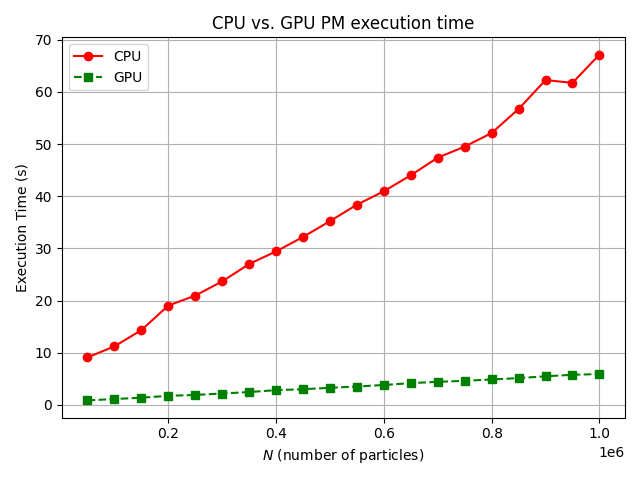
\includegraphics[scale=0.6]{img/cpu-vs-gpu.png}
    \caption{PM method: CPU and GPU implementation running time comparison.}
    \label{fig:cpu-vs-gpu-pm}
\end{figure}
In the test, the computational domain was split into $64\times 64 \times 32$ cells, and the simulation was run for 200 iterations.
Both plots in the figure exemplify linear complexity of the PM method, with the GPU implementation providing 1200\% speedup over the CPU version.
\chapter{Particle-particle particle-mesh method}
The \PThreeM{} algorithm is a hybrid method:
Forces between distant particles are calculated using the PM method, whereas, for particles lying closely together, the PP method is used.
The total force applied to particle $i$ is
\begin{equation}\label{eq:p3m}
    \mathbf{F}_i^\text{SR} + \mathbf{F}_i = \sum_{j \neq i}(\mathbf{f}_{ij}^\text{tot} - \mathbf{R}_{ij}) + \mathbf{F}_i,
\end{equation}
where $\mathbf{F}_i \approx \sum_{j\neq i} \mathbf{R}_{ij}$ is the force computed using the PM method and $\mathbf{R}_{ij} = \mathbf{R}(\mathbf{x}_i - \mathbf{x}_j)$ is a prescribed \textit{reference force}.
The reference force is defined as the force between two particle-clouds, i.e. each particle is represented by a sphere with diameter $a$ and a given density profile.
The two examples of reference forces described in \cite{Hockney1988} are
\begin{equation*}
    R(r) =
    G m_1 m_2 \times\begin{cases}
        \frac{1}{35 a^2} (224 \xi - 224 \xi^3 + 70 \xi^4 + 48 \xi^5 - 21 \xi^6),                               & 0 \leq \xi \leq 1 \\
        \frac{1}{35 a^2} (12 / \xi^2 - 224 + 896 \xi - 840 \xi^2 + 224 \xi^3 + 70 \xi^4 - 48 \xi^5 + 7 \xi^6), & 1 < \xi \leq 2    \\
        \frac{1}{r^2},                                                                                         & \xi > 2
    \end{cases}
\end{equation*}
where $\xi = 2r/a$ for a sphere with uniformly decreasing density (shape $S_2$) and
\begin{equation}\label{eq:s1-reference-force}
    R(r) =
    G m_1 m_2 \times\begin{cases}
        \frac{1}{a^2} (8 r / a - 9 r^2 / a^2 + 2 r^4 / a^4), & r < a \\
        \frac{1}{r^2},
    \end{cases}
\end{equation}
for a solid sphere (shape $S_1$).
The reference force vector lies along the line joining the two bodies.

\section{Optimal Green's function}
As it is apparent from \autoref{eq:p3m}, the method's validity depends on how well the mesh force approximates the reference force.
The average deviation between the two forces can be minimized by a suitable choice of the Green's function given (in $k$ space) by
\begin{equation}\label{eq:optimal-greens-func}
    \hat{\mathcal{G}}(\mathbf{k}) = \frac{\mathbf{\hat{D}}(\mathbf{k}) \cdot \sum_{\mathbf{n}}\hat{U}^2(\mathbf{k_\mathbf{n}}) \mathbf{\hat{R}}(\mathbf{k}_\mathbf{n})}{|\mathbf{\hat{D}}(\mathbf{k})|^2 \left[ \sum_{\mathbf{n}}\hat{U}^2(\mathbf{k}_\mathbf{n}) \right]^2}.
\end{equation}
The derivation is mathematically involved and is detailed in \cite{Hockney1988}.
We now proceed to examine the terms appearing in \autoref{eq:optimal-greens-func}.

\subsection{Finite difference operator}
The Fourier transform $\mathbf{\hat{D}}$ of the two-point finite difference operator defined in \autoref{eq:two-point-central-diff} has the components
\begin{align*}
    \hat{D}_j(\mathbf{k})
     & = \int D_j(\mathbf{x}) e^{-i\mathbf{k}\cdot \mathbf{x}} d\mathbf{x}                                                                                                                                      \\
     & = \frac{1}{2H}\left( \int \delta(\mathbf{x} + H\mathbf{e}_j)e^{-i \mathbf{k}\cdot \mathbf{x}} d\mathbf{x} - \int \delta(\mathbf{x} - H\mathbf{e}_j)e^{-i \mathbf{k}\cdot \mathbf{x}} d\mathbf{x} \right) \\
     & = \frac{1}{2H} (e^{ik_j H} - e^{-ik_j H})
    = \frac{i \sin(k_j H)}{H}.
\end{align*}
Similarly, for the four-point finite difference (\autoref{eq:four-point-central-diff}) we have
\begin{equation*}
    \hat{D}_j = \alpha\frac{i\sin k_j H}{H} + (1- \alpha)\frac{i\sin 2k_j H}{2H},
\end{equation*}
where $j=1,2,3$.

\subsection{Assignment function}
The quantity $\hat{U}$ is defined as $\hat{W}/V$.
For the mass assignment scheme hierarchy described in \autoref{sec:mass-assignment} we have
\begin{equation*}
    \hat{U}(\mathbf{k}) = \left(\prod_{i=1}^{3}\frac{\sin(k_i H / 2)}{k_i H / 2}\right)^{p},
\end{equation*}
where $p=1,2,3,\dots$, with $p=1$ corresponding to NGP assignment, etc.
In particular, for the TSC assignment scheme, the \textit{alias sum}
\begin{equation*}
    \sum_{\mathbf{n}}\hat{U}^2(\mathbf{k}_\mathbf{n})
    \equiv \sum_{\mathbf{n}}\hat{U}^2\left(\mathbf{k} + \mathbf{n}\frac{2\pi}{H}\right)
\end{equation*}
can be rewritten as
\begin{align*}
    \sum_{\mathbf{n}} \hat{U}^2\left(\mathbf{k}+\mathbf{n}\frac{2\pi}{H}\right)
     & = \sum_{\mathbf{n}} \prod_{i=1}^{3} \left[ \frac{\sin(k_i H/2 + n_i\pi)}{k_i H/2 + n_i\pi} \right]^6 \\
     & = \prod_{i=1}^{3} \sum_{n_i} \left[ \frac{\sin(k_i H/2 + n_i \pi)}{k_i H/2 + n_i \pi} \right]^6      \\
     & = \prod_{i=1}^{3} \left[ \sin^6\left(\frac{k_i H}{2}\right)
        \sum_{n_i} \frac{1}{(k_i H/2 + n_i \pi)^6} \right]
\end{align*}
Using the partial fractions expansion of the cotangent function \cite{aigner2018proofs},
\begin{equation*}
    \frac{(-1)^s}{s!}\frac{d^s}{dx^s}\cot x = \sum_{n=-\infty}^{\infty} \frac{1}{(x-n\pi)^{s+1}},
\end{equation*}
we can simplify the sum over $n_i$ to
\begin{equation*}
    \frac{-1}{5!} \frac{d^5}{dx^5}\cot\left( \frac{k_i H}{2} \right)
    = 1 - \sin^2\frac{k_i H}{2} + \frac{2}{15}\sin^4\frac{k_i H}{2}.
\end{equation*}
Hence,
\begin{equation*}
    \sum_{\mathbf{n}}\hat{U}_\text{TSC}^2(\mathbf{k}_\mathbf{n})
    = \prod_{i=1}^{3} \left(1 - \sin^2\frac{k_i H}{2} + \frac{2}{15}\sin^4\frac{k_i H}{2}\right).
\end{equation*}
Using the same approach, we can obtain similar results for the CIC and NGP schemes, namely
\begin{equation*}
    \sum_{\mathbf{n}}\hat{U}_\text{CIC}^2 = \frac{1}{27} \prod_{i=1}^{3} \left(1 + 2\cos^2\frac{k_i H}{2}\right)
    \quad \text{and} \quad
    \sum_{\mathbf{n}}\hat{U}_\text{NGP}^2 = 1.
\end{equation*}

\subsection{Reference force}
The quantity $\mathbf{\hat{R}}$, the transformed reference force, is related to the shape $S$ of the particle-cloud by
\begin{equation}\label{eq:reference-force-transform}
    \mathbf{\hat{R}}(\mathbf{k}) = \frac{i\mathbf{k}\hat{S}^2(k)}{k^2},
\end{equation}
where $k = |\mathbf{k}|$.
This can be shown by recalling that $\mathbf{R}(\mathbf{x}_i - \mathbf{x}_j)$ is the force applied to cloud $i$ due to cloud $j$.
Hence, $\mathbf{R}(\mathbf{x})$ is the force on the cloud centered at $\mathbf{x}$ due to a cloud at the origin.
The force acting on mass element $d\mathbf{x}' S(\mathbf{x}' - \mathbf{x})$ of the cloud centered at $\mathbf{x}$ is therefore
\begin{equation*}
    -G d\mathbf{x}'S(\mathbf{x}' - \mathbf{x}) \int d\mathbf{x}'' S(\mathbf{x}'')\frac{\mathbf{x}' - \mathbf{x}''}{|\mathbf{x}' - \mathbf{x}''|^3}
\end{equation*}
and the total force is
\begin{equation}\label{eq:reference-force-clouds}
    \mathbf{R}(\mathbf{x}) = -G \int d\mathbf{x}'S(\mathbf{x}' - \mathbf{x}) \int d\mathbf{x}'' S(\mathbf{x}'')\frac{\mathbf{x}' - \mathbf{x}''}{|\mathbf{x}' - \mathbf{x}''|^3}.
\end{equation}
The expression on the right-hand side of \autoref{eq:reference-force-clouds} is a double convolution, $\mathbf{R} = -G S * (S * \mathbf{g})$, where $\mathbf{g}(\mathbf{x}) = \mathbf{x}/|\mathbf{x}|^3.$
The $x$-coordinate of $\mathbf{g}$ is $x/|\mathbf{x}|^3$ which coincides with $\partial h / \partial x$ for $h(\mathbf{x}) = -1/|\mathbf{x}|.$
The Fourier transform of $h$ is given in \cite{gelfand1964generalized} (p. 363):
\begin{equation*}
    \hat{h}(\mathbf{k}) = \frac{4\pi}{|\mathbf{k}|^2}.
\end{equation*}
The formula for the transform of a derivative yields
\begin{equation*}
    \hat{g}_x(\mathbf{k}) = \frac{4\pi i k_x}{|\mathbf{k}|^2}.
\end{equation*}
Applying the convolution theorem twice and factoring the constant $(-4\pi G)$ out of the Green's function in \autoref{eq:optimal-greens-func} leaves us with the desired \autoref{eq:reference-force-transform}.

Since the shapes $S$ are spherically symmetric, the calculation of $\hat{S}$ (appearing in \autoref{eq:reference-force-transform}) can be simplified.
The Fourier transform of $S$ is
\begin{equation*}
    \hat{S}(\mathbf{k}) = \int d\mathbf{x} S(\mathbf{x}) e^{-i\mathbf{k} \cdot \mathbf{x}}.
\end{equation*}
Observe that $\mathbf{k} \cdot \mathbf{x} = kr\cos\theta$, where $\theta$ is the angle between $\mathbf{k}$ and $\mathbf{x}$, and $r = |\mathbf{x}|$.
Since $S$ is invariant under rotations, $\theta$ can be chosen to be the angle between $\mathbf{x}$ and the $z$-axis.
Thus, the integral, rewritten in spherical coordinates, becomes
\begin{equation*}
    \hat{S}(k) = \int_{0}^{2\pi}d\phi \int_{0}^{\pi} d\theta \int_{0}^{\infty}dr S(r)e^{-ikr\cos\theta}r^2\sin\theta
    = 2\pi \int_{0}^{\infty} r^2 dr \int_{0}^{\pi} d\theta e^{-ikr\cos\theta} \sin\theta.
\end{equation*}
The $\theta$-integral upon the substitution $-kr\cos\theta \to u$ becomes
\begin{equation*}
    \frac{1}{kr}\int_{-kr}^{kr} e^{iu} du
    = \frac{1}{kr} \int_{-kr}^{kr} (\cos u + i \sin u) du
    = \frac{2\sin kr}{kr}
\end{equation*}
and hence
\begin{equation*}
    \hat{S}(k) = 4\pi \int_{0}^{\infty} r^2 S(r)\frac{\sin kr}{kr}dr.
\end{equation*}

This integral, evaluated for the $S_1$ and $S_2$ shapes respectively, gives
\begin{equation*}
    \hat{S_1}(k) = \frac{3}{(ka/2)^3} \left(\sin\frac{ka}{2} - \frac{ka}{2} \cos\frac{ka}{2}\right)
\end{equation*}
and
\begin{equation*}
    \hat{S_2}(k) = \frac{12}{(ka/2)^4}\left(2 - 2\cos\frac{ka}{2}-\frac{ka}{2}\sin\frac{ka}{2}\right).
\end{equation*}

Finally, we note that the infinite sum in the numerator of \autoref{eq:optimal-greens-func} does not have a closed form, but this does not pose a problem since the summand decays rapidly with $\mathbf{n}$ moving further away from zero.

The result of applying the optimal Green's function in \autoref{eq:poisson-fourier-product} is illustrated in \autoref{fig:reference-force-combined}\subref{fig:reference-force-approx-sub}.
As can be seen, the PM force closely follows the reference force, especially for distances \( r > a \), where the reference force nearly matches the inverse-square law.
It is worth noting that for \( r \) slightly smaller than \( a \), the reference force and its mesh-based PM approximation still provide a good fit to the inverse-square behavior.
This observation allows the \textit{cutoff radius} \( r_e \), which defines the boundary for direct summation, to be chosen smaller than \( a \) (e.g., \( r_e = 0.7a \)), improving performance without sacrificing accuracy.
\begin{figure}[htp]
    \centering
    \begin{subfigure}[b]{0.48\textwidth}
        \centering
        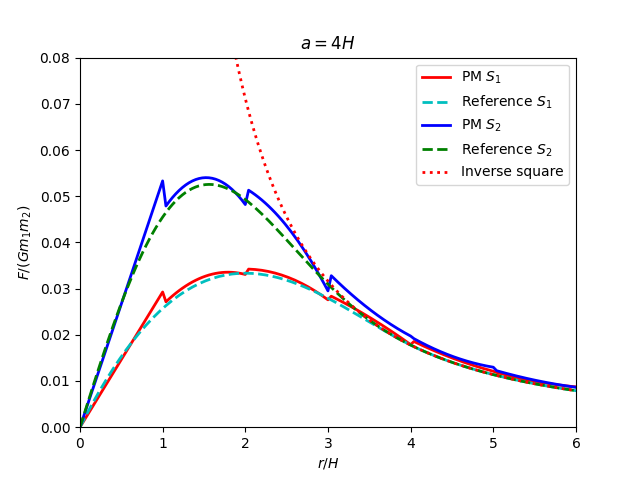
\includegraphics[width=\textwidth]{chapters/p3m-method/img/s1-vs-s2.png}
        \caption{Approximate vs. reference force.}
        \label{fig:reference-force-approx-sub}
    \end{subfigure}
    \hfill
    \begin{subfigure}[b]{0.48\textwidth}
        \centering
        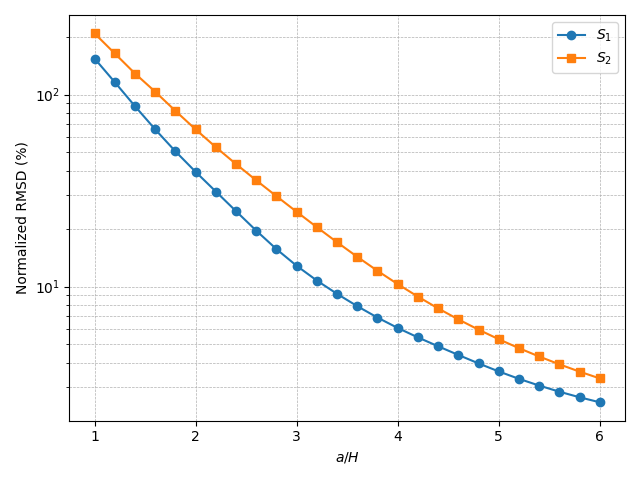
\includegraphics[width=\textwidth]{chapters/p3m-method/img/s1-vs-s2-nrmsd.png}
        \caption{Mean-normalized RMSD error}
        \label{fig:reference-force-error-sub}
    \end{subfigure}
    \caption{Comparison of PM approximation using $S_1$ and $S_2$ shape functions.
        The mesh approximation to the reference force was computed using the PM method with a TSC assignment scheme, two-point finite difference, and Green's function optimal for each shape.
    }
    \label{fig:reference-force-combined}
\end{figure}

\subsection{Error analysis}\label{subsec:p3m-error-analysis}
The \PThreeM{} method offers a high degree of flexibility in terms of specifying the ``building blocks'' of the Green's function in \autoref{eq:optimal-greens-func}.
For example, we can be interested in learning how the choice of the assignment scheme influences the shape of the PM-approximated reference force.
The result of a test that addresses this issue is shown in \autoref{fig:reference-force-approx-different-schemes}.
\begin{figure}[htp]
    \centering
    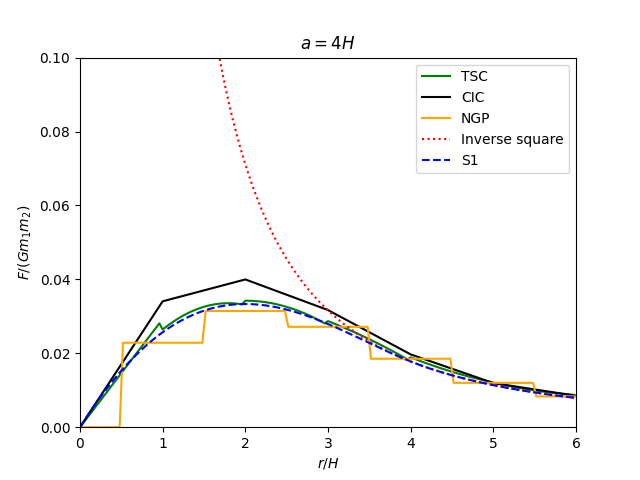
\includegraphics[scale=0.5]{chapters/p3m-method/img/field_different_ass.png}
    \caption{Approximate vs. reference force.}
    \label{fig:reference-force-approx-different-schemes}
\end{figure}
The figure shows that the general characteristic of the field strength approximated by the PM method is similar to what we have already seen in \autoref{fig:pm-mass-assignment-field-strength}.
Namely, the NGP scheme yields an unnatural, jagged shape.
The shape produced using the CIC shape matches the $S_1$ reference force more closely, although it overestimates the field strength values close to the source.
The most accurate approximation is obtained using the TSC scheme (this is the same shape we have already seen in \autoref{fig:reference-force-approx-sub}).


To measure the quality of PM-approximation of a given reference force, we used mean-normalized RMSD error, i.e., we calculated
\begin{equation*}
    \frac{\sqrt{\frac{1}{n} \sum_{i=1}^{n} (F^\text{PM}(r_i) - R(r_i))^2}}{\frac{1}{n} \sum_{i=1}^{n} R(r_i)}
\end{equation*}
in a system with a single unit mass located on the $x$-axis.
The forces $F^\text{PM}(r_i)$ were measured along the $x$-axis in equal-length intervals, and the test was run for increasing values of particle diameter $a$.
The result of the test is shown in \autoref{fig:reference-force-error-sub}.
Clearly, the approximation error becomes smaller for increasing values of $a$.
Since $r_e$ is proportional to $a$, this implies that there is a trade-off between accuracy and the execution time.
Increasing $a$ means that $r_e$ should increase as well, which forces more particles into short-range correction regions.
If in the system under consideration the particles are uniformly distributed, then for any given particle, the short-range correction is performed based on $\sim r_e^3$ particles in its vicinity, which translates into $\sim N r_e^3$ total operations.
The relation between cutoff radius size $r_e$ and execution time is shown in \autoref{fig:p3m-time-vs-radius}.
\begin{figure}[htp]
    \centering
    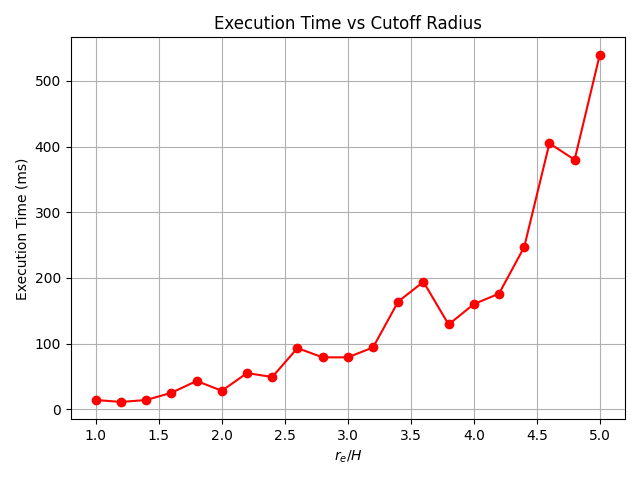
\includegraphics[scale=0.5]{chapters/p3m-method/img/time-vs-radius.png}
    \caption{Execution time for different settings of cutoff radius $r_e$ in the \PThreeM{} method (single step, $N=10{,}000$).
    The times shown in the graph do not include tabulating the Green's function and the PM step.}
    \label{fig:p3m-time-vs-radius}
\end{figure}
As we can see, the execution time very strongly depends on $r_e$, and this explains why choosing $r_e$ even slightly less than $a$ can lead to significant improvements in performance.
Another conclusion that can be drawn from \autoref{fig:reference-force-error-sub} is that the \( S_2 \)-based approximation exhibits higher mean-normalized RMSD error compared to \( S_1 \).
However, as we remarked previously, it allows for choosing $r_e \lesssim a$ without significant loss of accuracy.
Therefore, the choice between \( S_1 \) and \( S_2 \) shapes involves a trade-off between accuracy near the source and overall error, making the optimal choice context-dependent.


\section{Identifying close pairs of particles}
In the \PThreeM{} method, in addition to the mesh used in the PM algorithm (the ``potential mesh''), a second mesh (the \textit{chaining mesh}) is used.
The chaining mesh is sparser than the potential mesh.
Its sole purpose is to partition the space into cells so that particles ``close'' to the ones in a given cell can be found efficiently.
In this context, two particles are considered to lie close to one another if their separation is less than the cutoff radius.

The number of chaining mesh cells in a single dimension is given by $M_i = \lfloor L_i / r_e \rfloor$, where $L_i$ is the side length of the computational box ($i=1,2,3$).
This implies that the side length of a chaining mesh cell is $\text{HC}_i = L_i / M_i \geq r_e$.
Thus, for every particle $i$ in a given cell $\mathbf{p}$, it is sufficient to search through the immediate neighborhood of $\mathbf{p}$ to find all the particles within the cutoff radius from $i$.

In our program, the chaining mesh is implemented as a \textit{head-of-chain} (HOC) array, depicted in \autoref{fig:hoc}.
\begin{figure}[htp]
    \centering
    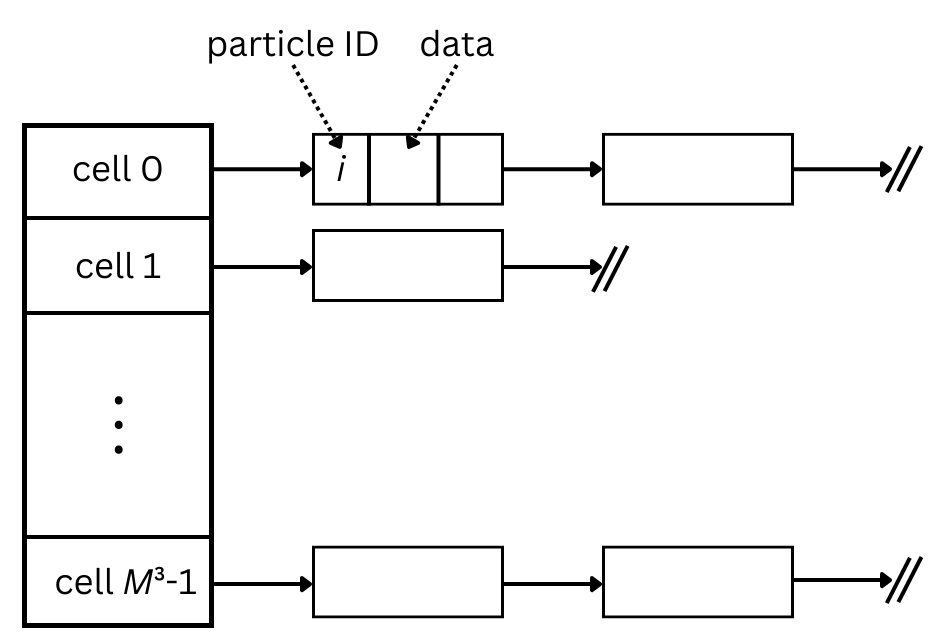
\includegraphics[scale=0.25]{chapters/p3m-method/img/hoc.png}
    \caption{Head-of-chain data structure used for mapping particles to their parent cells in the chaining mesh.
        Here $M_1=M_2=M_3 = M$.}
    \label{fig:hoc}
\end{figure}
The basic version of the HOC array is very cheap to build.
Given a particle at point $\mathbf{x} = (x, y, z)$, we can determine in which chaining mesh cell $\mathbf{c}$ it lies by simply performing integer division on each of its coordinates, i.e. $\mathbf{c} = (x / \text{HC}_1, y / \text{HC}_2, z / \text{HC}_3)$.
Then, to get a HOC table index $i$ corresponding to $\mathbf{c}$, standard index flattening is used.
Subsequently, a new linked-list node is allocated and inserted at the beginning of the list HOC[$i$].
Clearly, the whole process is linear in the number of particles and the array can be constructed anew at each time step without degrading performance.
In our implementation, additional savings are made by preallocating a memory pool large enough to store $N$ nodes of the linked lists and reusing it for the HOC array initialization.

A potential optimization discussed in \cite{Hockney1988} involves sorting each linked list by a selected particle coordinate, such as the $y$-coordinate.
This ordering enables early termination of the direct summation loop when the condition $y_i - y_j > r_e$ is met, effectively reducing unnecessary pairwise computations as particle $i$ "sweeps through" a cell containing particles $j$.
Our experiments indicate that constructing the linked lists in sorted order is substantially more expensive than the unsorted variant.
This is to be expected; in the worst-case scenario where all particles are in a single chaining-mesh cell, and are inserted into the list in decreasing order of $y$ coordinates, the complexity is $O(N^2)$.
For a system of 50{,}000 particles, incorporating $y$-sorting increased the HOC (head-of-chain) construction time from approximately 180 milliseconds to over 13{,}000 milliseconds, a 70-fold slowdown.
Despite this added cost, we observed no significant performance improvement in the short-range correction phase of the computation.

\section{Short-range correction}
The short-range correction, which takes place immediately after the mesh forces are found using the PM method, is at the heart of the \PThreeM{} algorithm.
Since it scales with a square of the number of particles in each neighborhood, further optimizations are highly desirable.

By Newton's 3rd law, $\mathbf{f}^\text{SR}_{ji} = -\mathbf{f}^\text{SR}_{ij}$, which allows us to do the calculation of the short-range inter-particle force for any pair $(i, j)$ of particles only once, leading to the reduction of the total running time by half.
Informally, the particle $i$ updates its total short-range force $\mathbf{F}^\text{SR}_i$ as well as the total short-range force $\mathbf{F}^\text{SR}_j$ of its neighbor $j$.
To avoid double-counting, the particle $i$ residing in cell $\mathbf{q}$ has to look for its neighbors in a subset $\mathcal{N}$ of the immediate neighborhood of $\mathbf{q}$.
More specifically, define
\begin{equation}\label{eq:n-set}
    \mathcal{N}(\mathbf{q} = (q_1, q_2, q_3)) = \{(q_1+t, q_2-1,q_3+s), (q_1+s, q_2, q_3-1), (q_1-1,q_2,q_3) \;|\; s,t = -1,0,1 \}.
\end{equation}
Thus $|\mathcal{N}| = 13$, which is half of the size of the immediate neighborhood.
The set $\mathcal{N}$ given in \autoref{eq:n-set} is not easily to illustrate.
Since for the purposes of the later discussion, it is beneficial to have a clear picture in mind, we depict its two-dimensional analog in \autoref{fig:n-set-2d}.
\begin{figure}[htp]
    \centering
    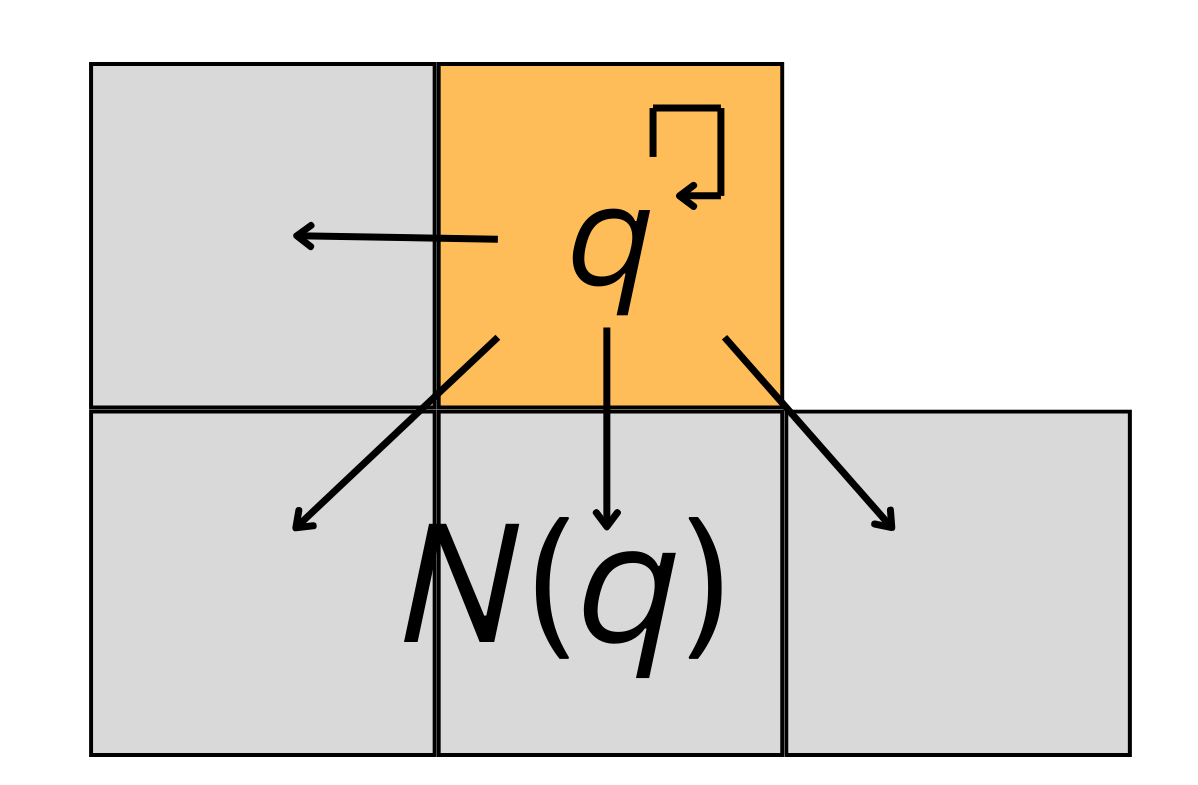
\includegraphics[scale=0.12]{chapters/p3m-method/img/q-neighborhood.png}
    \caption{Set $\mathcal{N}$ in two dimensions.}
    \label{fig:n-set-2d}
\end{figure}

The short-range correction part of the \PThreeM{} method is shown in \autoref{alg:short-range-correction}.
\begin{algorithm}
    \caption{Short-range correction}\label{alg:short-range-correction}
    \begin{algorithmic}[1]
        \ForAll {chaining cell $\mathbf{q}$}
        \ForAll {$\mathbf{q}_n \in \mathcal{N}(\mathbf{q}) \cup \{\mathbf{q}\}$}
        \ForAll {$i \in \text{HOC}(\mathbf{q})$}
        \ForAll {$j \in \text{HOC}(\mathbf{q}_n)$}
        \If {$|y_i - y_j| > r_e$}
        \Break
        \EndIf
        \State \Call{UpdateShortRange}{$i$, $j$, $\mathbf{q}$, $\mathbf{q}_n$}
        \EndFor
        \EndFor
        \EndFor
        \EndFor
    \end{algorithmic}
\end{algorithm}
For each chaining mesh cell $\mathbf{q}$, we compute the pair-wise interactions between the particles in $\mathbf{q}$ and the particles in the chaining mesh cells $\mathbf{q}_n$ from the reduced neighborhood $\mathcal{N}(\mathbf{q})$ \textit{plus} $\mathbf{q}$.
The inclusion of $\mathbf{q}$ allows us to take into account forces between particles within $\mathbf{q}$.

The \textsc{UpdateShortRange} procedure is defined in \autoref{alg:update-short-range-forces}.
\begin{algorithm}
    \caption{Updating short-range forces}\label{alg:update-short-range-forces}
    \begin{algorithmic}[1]
        \Procedure{UpdateShortRange}{$i$, $j$, $\mathbf{q}$, $\mathbf{q}_n$}
        \If {$i = j$}
        \Return
        \EndIf
        \State $\mathbf{r}_{ij} \gets \mathbf{r}_i - \mathbf{r}_j$
        \If {$|\mathbf{r}_{ij}|^2 > r_e^2$}
        \Return
        \EndIf
        \State $r_{ij} \gets |\mathbf{r}_{ij}|$
        \State $\mathbf{\hat{r}}_{ij} \gets \mathbf{r}_{ij} / r_{ij}$
        \State $\mathbf{R}_{ij} \gets -m_i m_j R(r_{ij}) \mathbf{\hat{r}}_{ij}$
        \State $\mathbf{f}^\text{tot} \gets -G m_i m_j / r_{ij}^2 \mathbf{\hat{r}}_{ij}$
        \State $\mathbf{f}^\text{SR}_{ij} \gets \mathbf{f}^\text{tot} - \mathbf{R}_{ij}$
        \State $\mathbf{f}^\text{SR}_{ji} \gets -\mathbf{f}^\text{SR}_{ij}$
        \State $\mathbf{F}^\text{SR}_i \gets \mathbf{F}^\text{SR}_i + \mathbf{f}^\text{SR}_{ij}$
        \If {$\mathbf{q}_n \neq \mathbf{q}$} \Comment{Avoid double-counting in the parent cell}
        \State $\mathbf{F}^\text{SR}_j \gets \mathbf{F}^\text{SR}_j + \mathbf{f}^\text{SR}_{ji}$
        \EndIf
        \EndProcedure
    \end{algorithmic}
\end{algorithm}
In line 2, we exclude self-forces.
The check in line 4 assures that the correction happens only for particles with separation less than the cutoff radius $r_e$.
The pair-wise short-range force is calculated in lines 5--10, with the calculation in line 10 exploiting the Newton's third law, as described previously.
The accumulation of total short-range force for a given particle takes place in line 11.
The short-range force is also added to the total short-range force of the other particle in the pair (particle $j$) but only if $\mathbf{q}_n \neq \mathbf{q}$.
This stipulation is crucial, as otherwise we would be double counting the forces between particles within $\mathbf{q}$.

As suggested in \cite{Hockney1988}, the computational burden of operations in lines 5--8 in \autoref{alg:update-short-range-forces} can be greatly reduced by storing the values of $f^\text{SR}(r) / r = (f^\text{tot}(r) - R(r)) / r$ in a lookup table $T$ at uniform intervals $\Delta^2$ of $[0, r_e^2]$ and interpolating them later.
The schematic depiction of the interpolation is shown in \autoref{fig:sr-force-val-interpolation}.
\begin{figure}[htp]
    \centering
    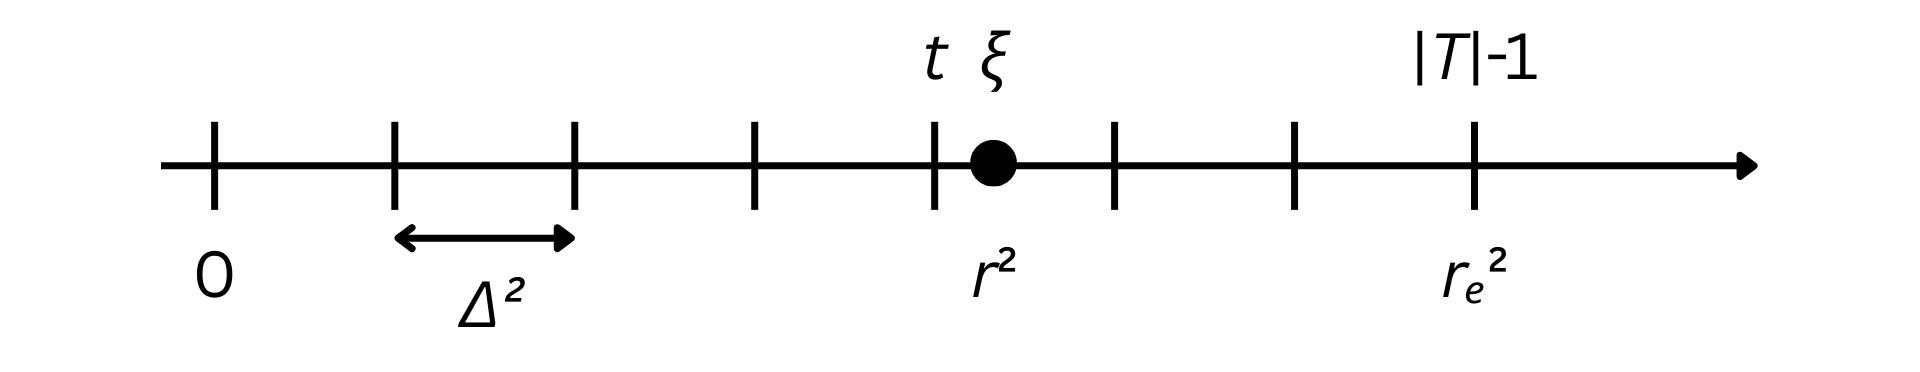
\includegraphics[scale=0.2]{chapters/p3m-method/img/interpolation.png}
    \caption{Interpolation of short-range force values.}
    \label{fig:sr-force-val-interpolation}
\end{figure}
If we define $\xi = r^2 / \Delta^2$ and $t=\lfloor \xi \rfloor$, then
\begin{equation*}
    \frac{f^\text{SR}(r)}{r} \approx T[t]\left(1 - (\xi - t)\right) + T[t+1](\xi - t)
    = T[t] + (\xi - t) (T[t+1] - T[t]).
\end{equation*}
The value $\mathbf{f}^\text{SR}_{ij}$ can then be obtained by multiplying the interpolated quantity $f^\text{SR}(r_{ij})/r_{ij}$ by $G m_i m_j \mathbf{r}_{ij}$, eliminating the use of the square root operations and reducing the total number of floating-point operations to just four.

In our implementation, the procedure outlined in\autoref{alg:short-range-correction} is parallelized by splitting the work done in the outmost loop between some number of threads.
In doing so, extra care has to be taken to avoid data races.
A thread $t$ that is currently processing cell $\mathbf{p}$ and its neighbors (we say that $t$ is \textit{assigned} to $\mathbf{p}$) may ``clash'' with a different thread assigned to a nearby cell $\mathbf{q}$ (because possibly $\mathbf{p} \in \mathcal{N}(\mathbf{q})$).
However, by the construction of the set $\mathcal{N}$, it is possible to split the short-range force into 14 parts, each of which is accessed by only one thread.
For example, consider a particle $i$ in cell $\mathbf{p} = (p_1, p_2, p_3)$ (in other words, $\mathbf{p}$ is the parent cell of $i$).
If thread $t$ is currently assigned to this cell, $t$ will update the part of $\mathbf{F}^\text{SR}_i$ corresponding to updates of $i$ coming from within the same cell as the parent cell of $i$.
Possibly at the same time, thread $t'$ assigned to cell $\mathbf{q} = (p_1+1, p_2, p_3)$ will update a different part of $\mathbf{F}^\text{SR}_i$, i.e. the part corresponding to updates of $i$ coming from the cell ``to the right'' of the parent cell of $i$.
Since only one thread is responsible for updates to particle $i$ coming ``from the right,'' (or any other ``direction'') no data races can occur.
This approach presents two major drawbacks.
First, it significantly increases memory usage, requiring storage for an additional $13N$ three-dimensional vectors.
Second, it offers no guarantee of uniform workload distribution across threads.
This imbalance, combined with the substantial variation in operations performed by individual threads, leads to severe thread divergence, rendering the parallelization scheme unsuitable for GPU execution.

\section{Force approximation error and performance}
The ``local picture'' of the errors of force approximation in the \PThreeM{} method has already been outlined in \autoref{fig:reference-force-combined}.
Now we turn to investigate how the choice of the particle shape ($S_1$ or $S_2$) and the size of the particle diameter influences the global force approximation error.
The error is defined exactly the same as in the case of the PM method, i.e. we use \autoref{eq:force-avg-relative-err}.

In our test, the grid covering the computational region had dimensions of $64\times 64\times 32$ and $N=10{,}000$ particles were used.
The result of the test is shown in \autoref{fig:p3m-global-err}.
\begin{figure}[htp]
    \centering
    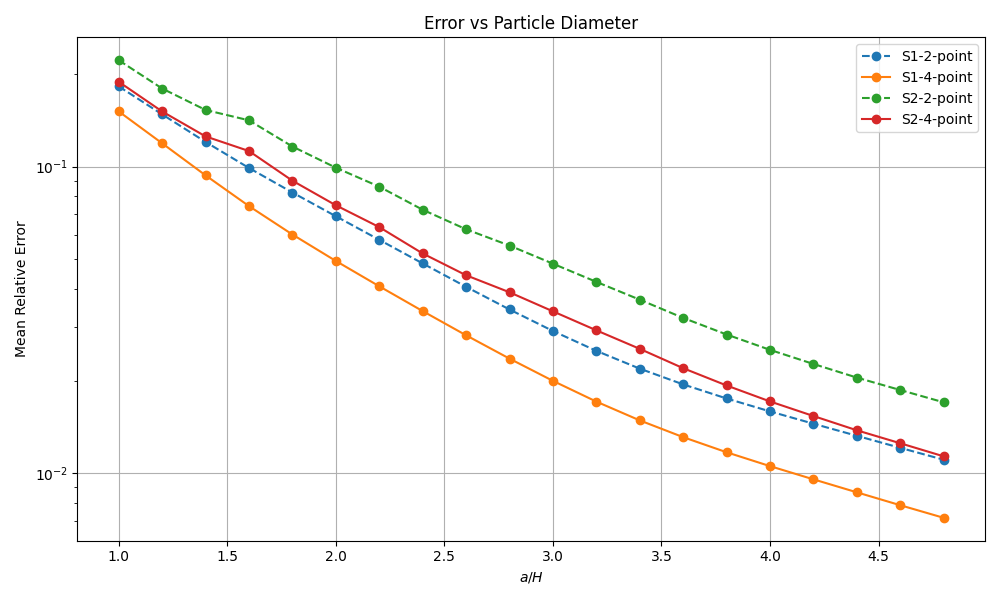
\includegraphics[scale=0.5]{img/err_vs_part_diam_p3m.png}
    \caption{Mean relative error in P3M approximation.}
    \label{fig:p3m-global-err}
\end{figure}
The figure clearly illustrates that the error drops with increasing the size of the particle diameter $a$.
This is an expected result, since with increasing $a$, the P3M method calculates more interparticle forces through exact direct summation.
Moreover, as we could see in \autoref{fig:reference-force-error-sub}, the PM approximation to the reference force gets better with increasing particle diameter.
These two effects combined are responsible for the reduction of the global error.

For both the $S_1$ and $S_2$ shapes, the error was minimized when the fourth-order finite difference was used for gradient calculation, as one could obviously expect.
The test indicated superiority of the $S_1$ shape, with the difference between the two becoming more significant for bigger relative values of $a$.


\chapter{Barnes-Hut algorithm}
The idea behind Barnes-Hut algorithm differs substantially from previously described mesh-based methods.
The algorithm deals with gravitational forces directly instead of deriving them from the mesh-defined potential, as was the case with the PM and \PThreeM{} methods.
Significant reduction of time complexity, from quadratic to $O(N \log N)$, is achieved by approximating the potential due to ``far enough'' groups of particles by the initial terms of its multipole expansion \cite{trenti2008gravitationalnbodysimulations}.
The grouping of particles is hierarchical in nature and is thus best understood as a tree.
The entire set of particles comprises the top-level group, represented by the root of the tree;
the eight children of the root node are representative of groups of particles residing in each of the octants of the computational domain, etc.
The process of subdividing the space into eight smaller volumes at each node continues recursively until there is only one or zero particles left in a given volume.
Nodes which satisfy this condition are the leafs of tree and are sometimes called the \textit{external nodes}.
The remaining nodes, each of which has eight children, are called \textit{internal nodes}.

In the basic variant of the algorithm, the potential due to a group of particles is approximated using only the monopole term with respect to the center of mass of the group, i.e.
\begin{equation*}
    \phi_\text{mon}(r) = -\frac{GM}{r},
\end{equation*}
where $M$ is the group's total mass.
Since the potential is expanded about the center of mass, the dipole moment $\mathbf{p} = \sum_{i} m_i \mathbf{r}_i$ vanishes.
Hence, the next possible improvement comes from including the quadrupole term
\begin{equation*}
    \phi_\text{quad}(r) = -\frac{G}{2r^5} \mathbf{r} \cdot (\mathbf{Q} \mathbf{r}),
\end{equation*}
where $\mathbf{Q}$ is the quadrupole moment tensor defined as
\begin{equation*}
    Q_{ij} = \sum_{k} (3r_{ki}r_{kj} - 3r_k^2\delta_{ij})m_k.
\end{equation*}
In theory, we could keep on adding more terms to improve the quality of the approximation.
In our implementation however, we restrict ourselves to the quadrupole term.

\section{Building the tree} % checked
The data structure that fits the description given in the introduction is called an \textit{octree}.
An internal node of the octree stores the COM vector, the total mass of the group it represents, and the quadrupole tensor, whereas an external node stores a reference to the actual particles (or is empty if no particle was found in its associated volume).
The recursive procedure of building the tree is shown in \autoref{alg:bh-tree-insert}.
\begin{algorithm}
    \caption{Insert a particle into the Barnes-Hut tree}\label{alg:bh-tree-insert}
    \begin{algorithmic}[1]
        \Function{Insert}{$n$, $p$}
        \If{$n$ is an internal node}
        \State Update $n.\textrm{COM}$ and total mass $n.M$ of $n$ with $p$
        \State \Call{Insert}{child of $n$ that should contain $p$, $p$}
        \ElsIf{$n$ is empty}
        \State Assign $p$ to $n$
        \Else \Comment{Occupied external node}
        \State Subdivide $n$ into child nodes
        \State Move existing particle $p'$ in $n$ into child that should contain $p'$
        \State Update center of mass and total mass of $n$ with $p$ and $p'$
        \State \Call{Insert}{child of $n$ that should contain $p$, $p$}
        \EndIf
        \EndFunction
    \end{algorithmic}
\end{algorithm}
The quadrupole moment tensor for each node is calculated once the whole tree is already built.
The recursive relation used in this calculation is given in \cite{hernquist1987performance} and reads
\begin{equation*}
    \mathbf{Q} = \sum_{\text{child }c} \mathbf{Q}_c + \sum_{\text{child }c} m_c(3 \mathbf{R}_c \otimes \mathbf{R}_c - R_c^2 \mathbf{I}),
\end{equation*}
where $\mathbf{R}_c = \mathbf{x}^\text{COM}_c - \mathbf{x}^\text{COM}$ is the displacement vector from the COM of child $c$ to the COM of the parent, $\mathbf{I}$ is the identity matrix, and $\otimes$ denotes the outer product.

For reasons that will become apparent later, it can be beneficial to separate the COM calculation from the tree creation part.
In such a case, the COM is calculated recursively using the relation
\begin{equation}\label{eq:bh-com-calculation}
    \mathbf{x}^\text{COM} = \frac{\sum_{\text{child } c} m_c \mathbf{x}_c^\text{COM}}{\sum_{\text{child } c} m_c}
\end{equation}
after the tree has already been built (and obviously before the quadrupole moment calculation).

\section{Acceleration calculation}
In the Barnes-Hut algorithm, the net acceleration of a particle $p$ is calculated by summing the contributions from single particles or groups of particles while traversing the tree.
The decision whether the acceleration can be approximated using the information stored in an internal node $n$ depends on the relative distance from $p$ to $n.\textrm{COM}$ (the center of mass of group represented by $n$).
The distance is relative to the \textit{width} $H$ of the node, i.e. the side length of the cubical volume encompassed by the node.
More concretely, the approximation takes place if $n.H / |n.\mathrm{COM} - p.\mathbf{x}| < \theta$, where $\theta$ is the so-called \textit{opening angle}.
In the extreme case when $\theta$ is set to zero, no approximations take place, and the algorithm reduces to the PP method.
The procedure described above is illustrated in \autoref{alg:bh-find-force}.
\begin{algorithm}
    \caption{Compute gravitational force on a particle using Barnes-Hut approximation}
    \label{alg:bh-find-force}
    \begin{algorithmic}[1]
        \Function{FindAcceleration}{$n$, $p$, $\theta$}
        \If{$n$ is an external node}
        \If{$n$ contains a particle $q \neq p$}
        \State $p.\mathbf{a} \gets p.\mathbf{a} + \Call{GravitySoft}{q.\mathbf{x}, q.m, p.\mathbf{x}} / p.\text{mass}$
        \EndIf
        \State \Return
        \EndIf
        \If{$n.H / |n.\text{COM} - p.\mathbf{x}| < \theta$}
        \State $p.\mathbf{a} \gets p.\mathbf{a} + \Call{Gravity}{n.\mathrm{COM}, n.M, p.\mathbf{x}}$
        \State \Return
        \EndIf
        \ForAll{child $n_c$ of $n$}
        \State \Call{FindAcceleration}{$n_c$, $p$, $\theta$}
        \EndFor
        \EndFunction
    \end{algorithmic}
\end{algorithm}
In the implementation, the \textsc{GravitySoft} function calculates the gravitational force softened by $\epsilon$, i.e. it returns the value given by \autoref{eq:softened-force}.
The pairwise potential energy associated with this force is given by
\begin{equation}\label{eq:pe-soft}
    \Phi_{ij}^\textrm{soft} = - \frac{G m_i m_j}{\sqrt{r_{ij}^2 + \epsilon^2}}.
\end{equation}
The \textsc{Gravity} function returns the approximation (up to the quadrupole term) of the acceleration due to a group of particles represented by a given node, i.e.
\begin{equation*}
    \mathbf{a} = -GM \frac{\mathbf{r}}{r^3} + \frac{G}{r^5}\mathbf{Q}\mathbf{r} - \frac{5G}{2}(\mathbf{r} \cdot (\mathbf{Q} \mathbf{r})) \frac{\mathbf{r}}{r^7}
\end{equation*}
(see \cite{hernquist1987performance}).

One possible way to quantify the quality of approximation for a given value of $\theta$ is to consider the relative error of calculated force.
We set the same initial conditions of the system for both the PP direct summation method and the Barnes-Hut algorithm, compute the deviation of Barnes-Hut forces from PP forces acting on each particle, and take the average over all particles.
In other words, the error calculated is given by the \autoref{eq:force-avg-relative-err}.
The dependence of the error on the opening angle $\theta$ and the corresponding execution time are shown in \autoref{fig:bh-analysis}.
The figure includes plots for two cases: when only the monopole term is used in the Barnes-Hut approximation, and when both the monopole and quadrupole terms are included.
As can be seen, the quadrupole-based algorithm exhibits significantly improved error scaling with increasing $\theta$.
Naturally, this raises the question of the additional computational cost incurred by the inclusion of the quadrupole term.
Our tests showed that this impact is minimal.
The results (for $N = 10{,}000$ particles and $0 \leq \theta \leq 2$) support this observation.
\begin{figure}[htp]
    \centering
    \begin{subfigure}[b]{0.47\textwidth}
        \centering
        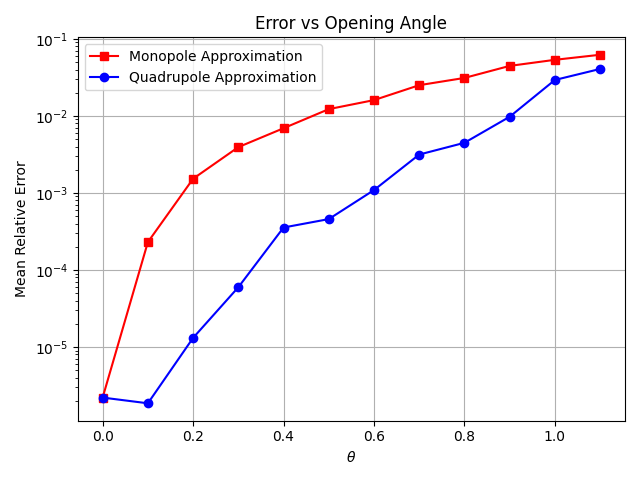
\includegraphics[width=\textwidth]{chapters/barnes-hut/img/error-vs-theta.png}
        \caption{Force approximation error.}
        \label{fig:bh-force-error}
    \end{subfigure}
    \hfill
    \begin{subfigure}[b]{0.47\textwidth}
        \centering
        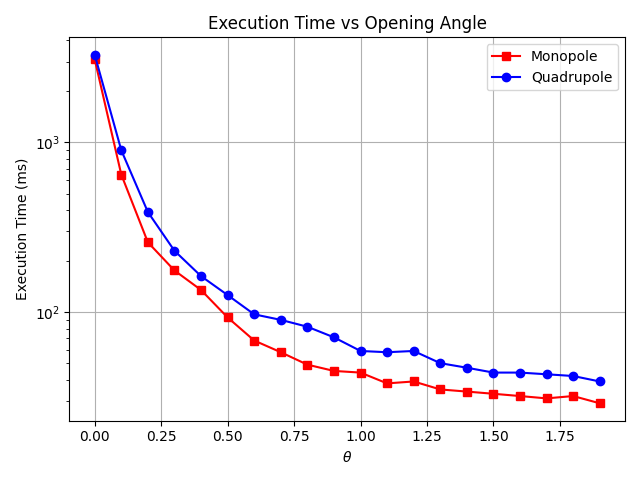
\includegraphics[width=\textwidth]{chapters/barnes-hut/img/bh-time.png}
        \caption{Execution time per iteration.}
        \label{fig:bh-time}
    \end{subfigure}
    \caption{Comparison of error and execution time in the Barnes-Hut algorithm using monopole and quadrupole approximations.}
    \label{fig:bh-analysis}
\end{figure}
Both tests described above were conducted on a uniform disk particle distribution.

We note that direct calculation of total potential energy is infeasible as $O(N^2)$ operations would be required.
Instead, we use an approximation based on the values stored in the tree.
The approximate value of the potential energy is accumulated for each particle using a procedure analogous to force calculation.
Indeed, the only difference between the two is the replacement of gravitational force calculation in \autoref{alg:bh-find-force} with potential energy calculation according to \autoref{eq:pe-soft}.

It is also noteworthy that the procedure outlined in \autoref{alg:bh-find-force} is embarrassingly parallel.
In our CPU implementation, the workload is split between an arbitrary number of threads on particle-by-particle basis.

\section{Accelerating tree construction}\label{sec:accelerating-tree-construction}
Unlike the force calculation part which is easily parallelized, the tree construction step is inherently sequential.
An approach to parallel tree construction outlined in \cite{warren_salmon_1993} involves splitting the set of particles into load-balanced spatial groups which are then used to construct separate trees (one per thread), with the final step being the merge of the created trees.
The merge step is highly involved and beyond the intended scope of this thesis.
For this reason, we propose an alternative approach to accelerating the tree construction which does not involve building the tree in parallel.

Our strategy, based on the ideas put forth in \cite{warren_salmon_1993}, stems from an observation that a potential bottleneck in \autoref{alg:bh-tree-insert} is related to irregular accesses to the nodes of the tree.
Inserting two particles separated by a large spatial distance leads to visiting nodes along two completely different paths in the tree which results in a huge number of cache misses.
A solution to this problem is to sort the list of particles in such a way that subsequent particles on the list (typically) lie close to each other in the physical space.
An ordering with this property can be generated by numbering the particles based on their position along a chosen \textit{space-filling curve}.

A space filling curve can be thought of as the limit of an infinite sequence of curves which ``fill'' the space without ``holes'' \cite{WeissteinPlaneFilling}.
In the limit, the curve reaches every point of the space, but due to practical constraints we can only deal with an approximation, i.e. some member of the limiting sequence.
In our implementation, we are working with a \textit{Z-order curve}, also called a \textit{Morton space-filling curve}, so it will in the focus of our discussion.
To make the visualization simpler, assume that the computational domain is two-dimensional and coarsely divided into 16 cells (particles within the same cells are ordered arbitrarily).
Then, the Z-order curve that covers all 16 cells is shown in \autoref{fig:z-order-curve}.
\begin{figure}[htp]
    \centering
    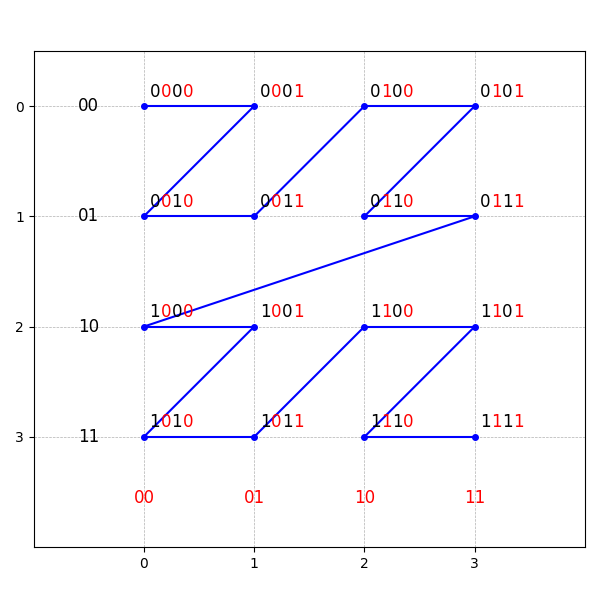
\includegraphics[scale=0.5]{chapters/barnes-hut/img/z-order.png}
    \caption{Z-order curve.}
    \label{fig:z-order-curve}
\end{figure}
The ordering of the points along the curve is obtained by assigning each cell a \textit{Z-value}, whose binary representation is calculated by interleaving the bits of the $x$ and $y$ coordinates.
This is illustrated in \autoref{fig:z-order-curve} by coloring the $x$- and $y$-coordinate bits red and black respectively.

In a standard setting, the coordinates of a particle are given by real numbers and not integers however.
In order to establish a mapping between the two, we have to first decide on the intended resolution of the grid.
In our implementation, we use the 32-bit integer type to represent the Z-values, which means that each coordinate should be represented by a 10-bit integer number ($3 \times 10 = 30 \leq 32$).
Thus, the mapping from real-valued coordinate of a particle to an integer one is given by
\begin{equation*}
    \left\lfloor \frac{(x - \text{low}.x)}{H} \times (2^{10} - 1)\right\rfloor \in [0, 2^{10}),
\end{equation*}
where $\text{low}$ and $H$ define the computational domain as
\begin{equation*}
    \text{domain} = [\text{low}.x, \text{low}.x + H] \times [\text{low}.y, \text{low}.y + H] \times [\text{low}.z, \text{low}.z + H].
\end{equation*}

In our proposed optimization, we make the following changes into the tree construction algorithm (\autoref{alg:bh-tree-insert}):
\begin{enumerate}
    \item The insertion does no longer start at the root of the tree for each particle but at the last inserted to node,
    \item The COM calculation is deferred until the tree construction is finished and carried out using \autoref{eq:bh-com-calculation}.
\end{enumerate}
The second point is a direct consequence of the first one;
if the insertion of a particle does not start at the root but at some other node $n$, deep in the tree, the nodes lying above $n$ will not be updated so their COM and total mass values will be incorrect.
The first point, however, requires more explanation.
Since the particles are z-ordered, subsequent inserts into the tree will result in traversing similar paths.
Because of that, the point of insertion can be found more efficiently by starting the traversal from the last seen node and backtracking up the tree until a valid insertion point is found.
The decision whether to stop backtracking at a given node $n$ is made on the condition that the particle to be inserted is inside a cube represented by $n$.
When the condition is met, the standard insertion procedure takes place starting at $n$.

The asymptotic time complexity of the modified tree construction algorithm is the same as for the standard one.
Sorting the particles requires $O(N\log N)$ operations but inserting a particle into the tree starting at the last-seen node is an $O(1)$ operation.
The last claim may raise objections, since some number of backtrack steps is expected on each insert.
To verify it, we measured the average number of backtracks per particle in typical simulations and found that it did not exceed $2.5$ (this can be compared with the number of backtracks required when the particles are not z-ordered; in such a case, we found that in the tested scenarios, on average more than 8 backtracks were typically needed).
Even though the modified algorithm still has the $O(N\log N)$ time complexity, it leads to more predictable memory access patterns which results in noticeably improved performance.
The tree construction time as a function of $N$ is shown in \autoref{fig:z-order-tree-time}.
\begin{figure}[htp]
    \centering
    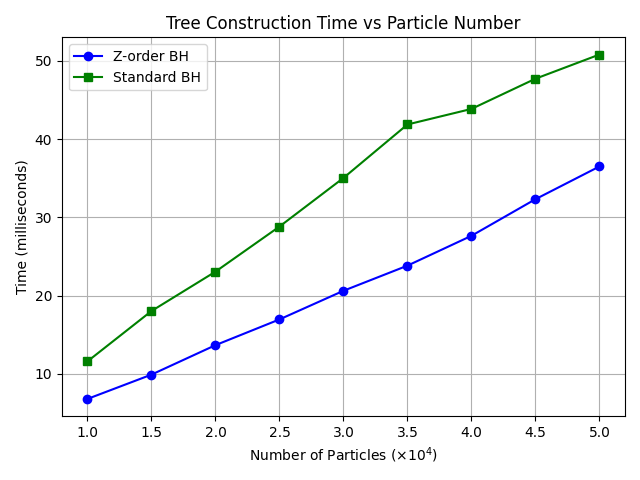
\includegraphics[scale=0.5]{chapters/barnes-hut/img/tree_construction_time.png}
    \caption{Tree construction time averaged over the number iterations of the simulation ($\theta = 1$).}
    \label{fig:z-order-tree-time}
\end{figure}
For the purposes of generating the graphs shown there, the tree construction time was measured in a spiral galaxy simulation.
As can be seen in the figure, the improved algorithm allows for up to $40\%$ speedup over the standard version.
In our tests, we used the standard library procedure \texttt{std::sort} with the parallel execution policy, which offered a slight speedup over the sequential variant.

\chapter{Time integration}
In the previous sections we described various methods of calculating forces applied to particles in the simulation.
Once these forces are found, the evolution of the system in time can be tracked by integrating Newton's 2nd law of motion,
\begin{equation}\label{eq:newtons-second}
    \ddot{\mathbf{x}}_i = \frac{\mathbf{F}_i}{m_i}.
\end{equation}

\section{Euler's method}
Possibly, the simplest numerical method that could be used is Euler's method described by the update rules
\begin{equation}\label{eq:eulers-method}
    \begin{aligned}
        \mathbf{v}_i^{(k+1)} & = \mathbf{v}_i^{(k)} + \textrm{DT} \frac{\mathbf{F}^{(k+1)}_i}{m_i}, \\
        \mathbf{x}_i^{(k+1)} & = \mathbf{x}_i^{(k)} + \textrm{DT} \mathbf{v}_i^{(k)},
    \end{aligned}
\end{equation}
where $\mathrm{DT}$ is the time step length.
The method defined in \autoref{eq:eulers-method} is not suitable for physical simulations, however.
Its shortcomings are well illustrated by an example of an undamped pendulum of length $l$ in a gravitational field of magnitude $g$.
Although it is a rudimentary system, it illustrates the numerical challenges faced in gravitational simulations over long timescales, particularly the issue of energy preservation.

The differential equation that governs the motion of the pendulum says
\begin{equation*}
    \ddot{\theta} = -\frac{g}{l}\sin\theta,
\end{equation*}
and the pendulum's kinetic and potential energy are given by $\textrm{KE} = (1/2)ml^2\dot{\theta}$ and $\textrm{PE} = -mgl\cos\theta$ respectively.
\begin{figure}[htp]
    \centering
    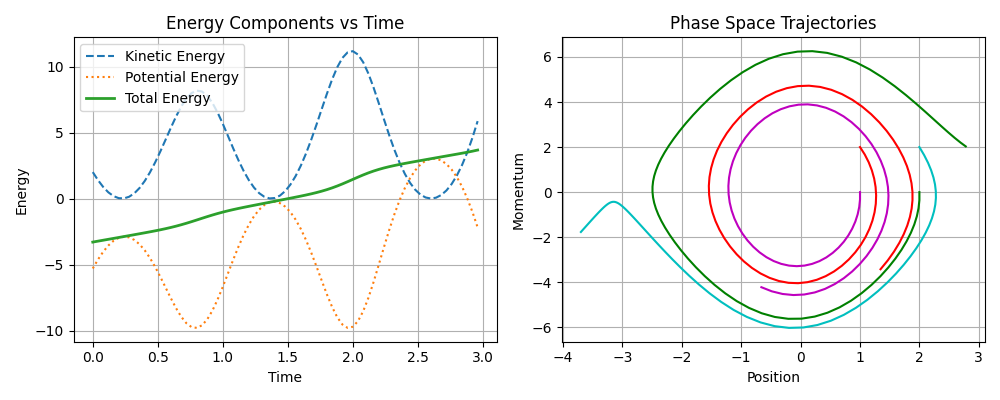
\includegraphics[scale=0.6]{chapters/time-integration/img/euler-pendulum.png}
    \caption{Behavior of Euler's method: lack of conservation of energy and phase space trajectories spiraling out.}
    \label{fig:euler-integrator}
\end{figure}
As shown in \autoref{fig:euler-integrator}, Euler's method fails to conserve total energy $(\textrm{PE} + \textrm{KE})$ and produces trajectories in phase space that are not closed, contrary to expectations for periodic systems.
Additionally, the evolution of an area element in phase space violates Liouville's theorem,\footnote{If we represent identical systems launched at the same time with slightly different initial conditions as points in phase space, then the theorem essentially states that the volume occupied by any group of such points stays constant.
    A more complete description of the theorem is given in \cite{taylor2005classical}.
}
making the method unsuitable for long-term physical simulations (see \autoref{fig:area-euler-vs-leapfrog}).
\begin{figure}[htp]
    \centering
    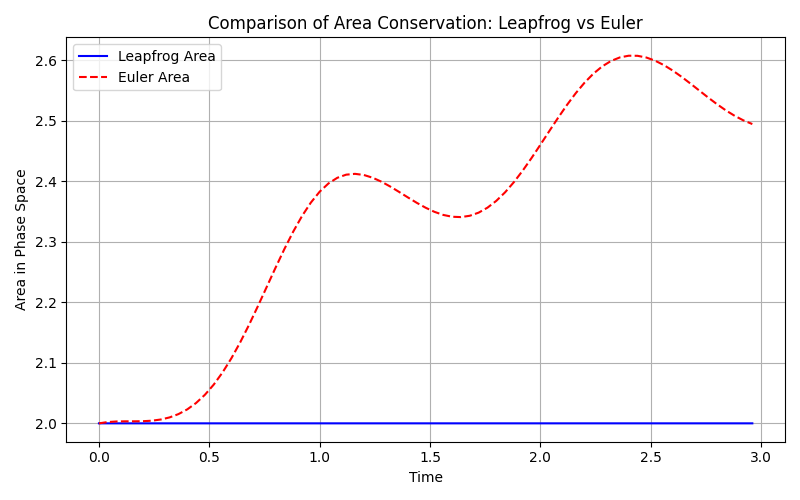
\includegraphics[scale=0.4]{chapters/time-integration/img/area-leap-vs-euler.png}
    \caption{Area in phase space over time. Violation of Liouville's theorem by Euler's method.}
    \label{fig:area-euler-vs-leapfrog}
\end{figure}
\section{Leapfrog algorithm}
The leapfrog algorithm, given by the update rule \cite{young_leapfrog_2019}
\begin{equation}\label{eq:leapfrog}
    \begin{aligned}
        \mathbf{v}_{i}^{(1/2)} & = \mathbf{v}_i^{(0)} + \frac{1}{2}\textrm{DT} \frac{\mathbf{F}_i^{(0)}}{ m_i^{(0)}}, \\
        \mathbf{x}_i^{(k+1)}   & = \mathbf{x}_i^{(k)} + \textrm{DT} \mathbf{v}_i^{(k+1/2)},                           \\
        \mathbf{v}_i^{(k+3/2)} & = \mathbf{v}_i^{(k+1/2)} + \textrm{DT} \frac{ \mathbf{F}_i^{(k+1)}}{m_i}.
    \end{aligned}
\end{equation}
is the preferred way of integrating \autoref{eq:newtons-second}.
When applied to the same pendulum system, it conserves energy much more faithfully. It preserves the area in phase space, consistent with Liouville's theorem (see \autoref{fig:leapfrog-integrator} and \autoref{fig:area-euler-vs-leapfrog}).
\begin{figure}[htp]
    \centering
    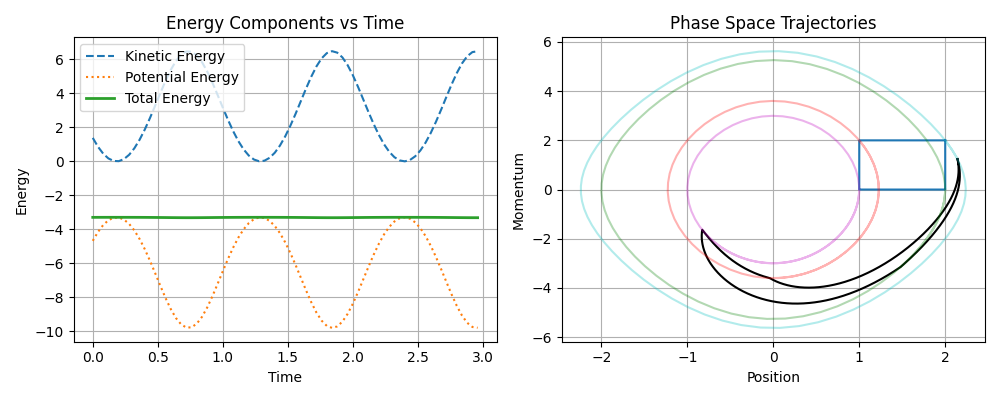
\includegraphics[scale=0.6]{chapters/time-integration/img/leapfrog-pendulum.png}
    \caption{Behavior of the leapfrog algorithm: conservation of energy and phase space trajectories forming closed loops.
        The evolution of an area element in phase space is shown on the right-hand side: blue rectangle -- initial conditions for many copies of the system; black distorted quadrilateral -- their state by the end of the simulation.}
    \label{fig:leapfrog-integrator}
\end{figure}
Given its simplicity and excellent long-term energy behavior, we adopt the leapfrog algorithm to integrate Newton's equations into our program.
\chapter{Test Models}

\section{Galaxy model}\label{sec:galaxy-model}
The model of a galaxy used as a test bed for the implementation is a simple one.
The galaxy is assumed to comprise only two parts: a thin disk and a spherically symmetric halo.
The disk comprises a large number of particles, each representing some number of stars.
The halo is simulated as a fixed external gravitational field.
The schematic illustration of the model is shown in \autoref{fig:galaxy-model}.
\begin{figure}[htp]
    \centering
    \begin{subfigure}[t]{0.45\textwidth}
        \centering
        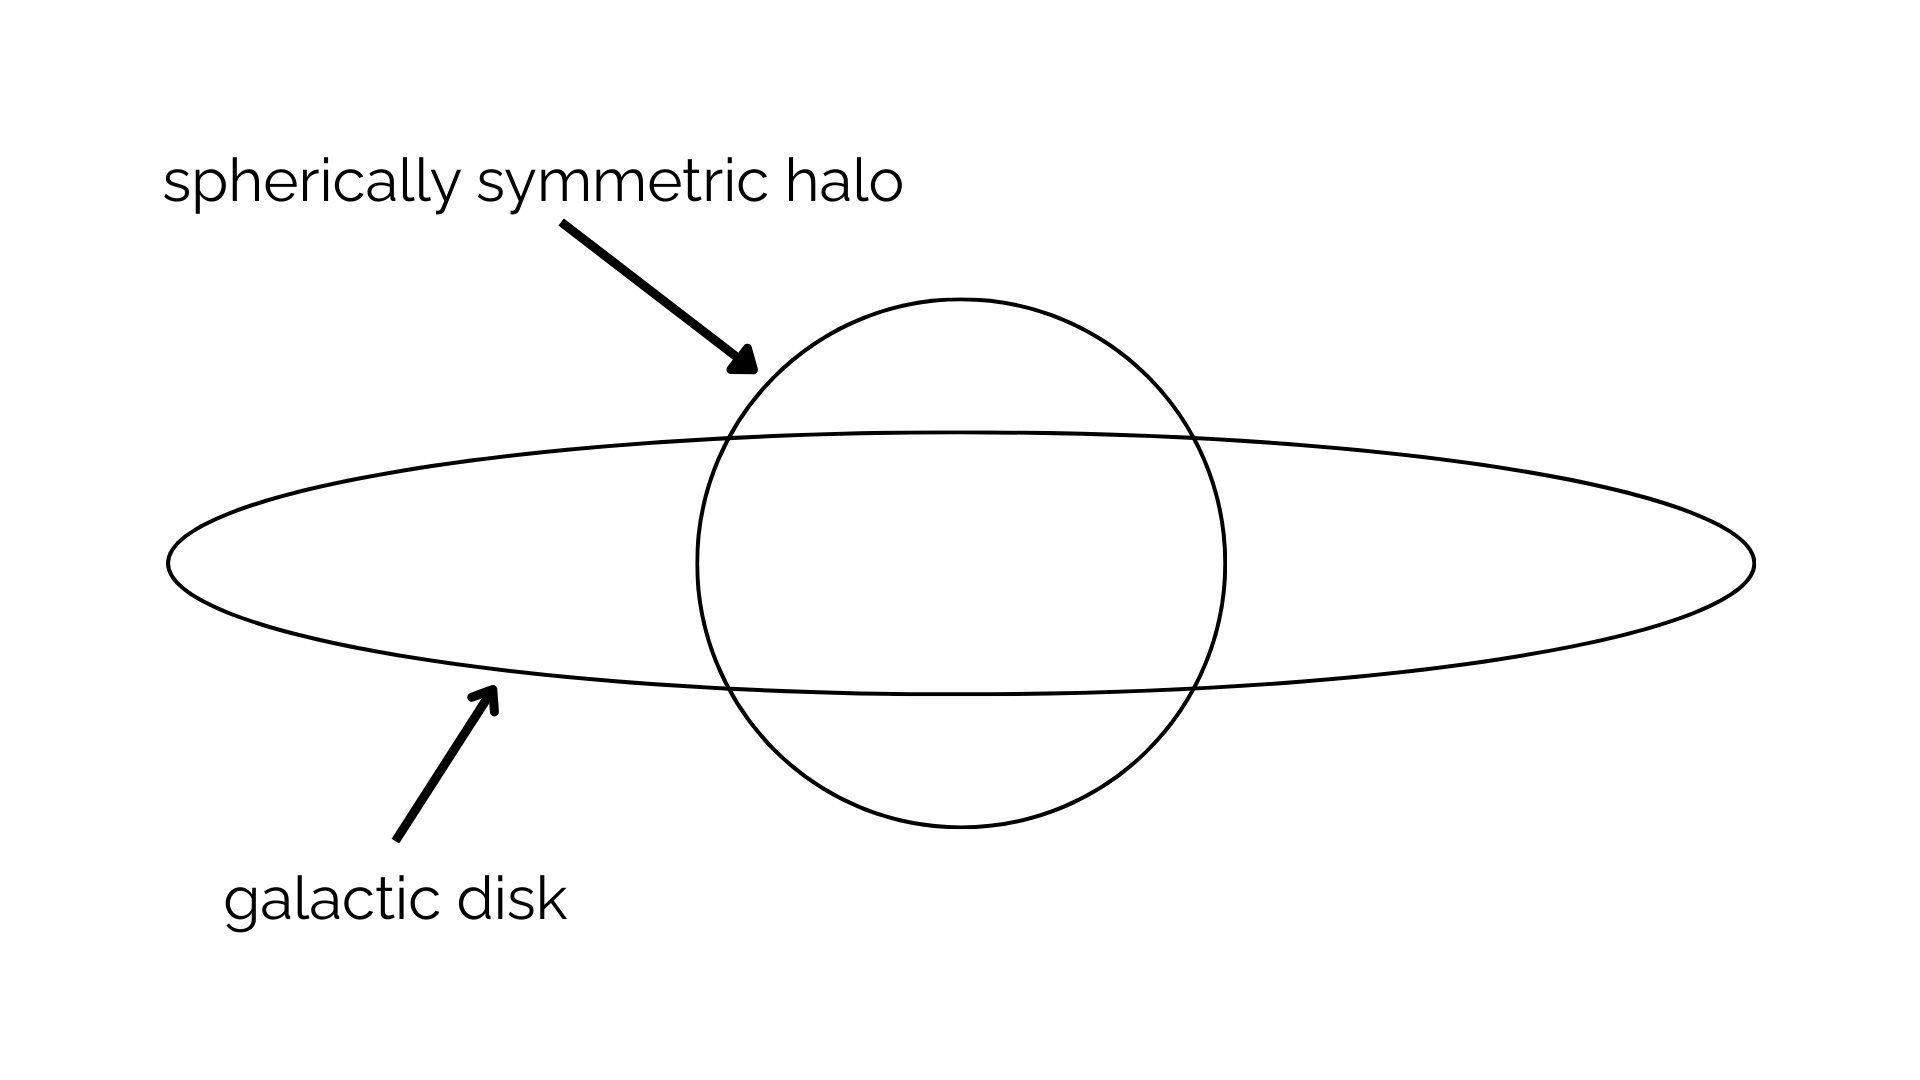
\includegraphics[scale=0.12]{chapters/test-models/img/galaxy-model.png}
        \caption{Spiral galaxy model (thin disk and spherical halo).}
        \label{fig:galaxy-model}
    \end{subfigure}
    \hfill
    \begin{subfigure}[t]{0.45\textwidth}
        \centering
        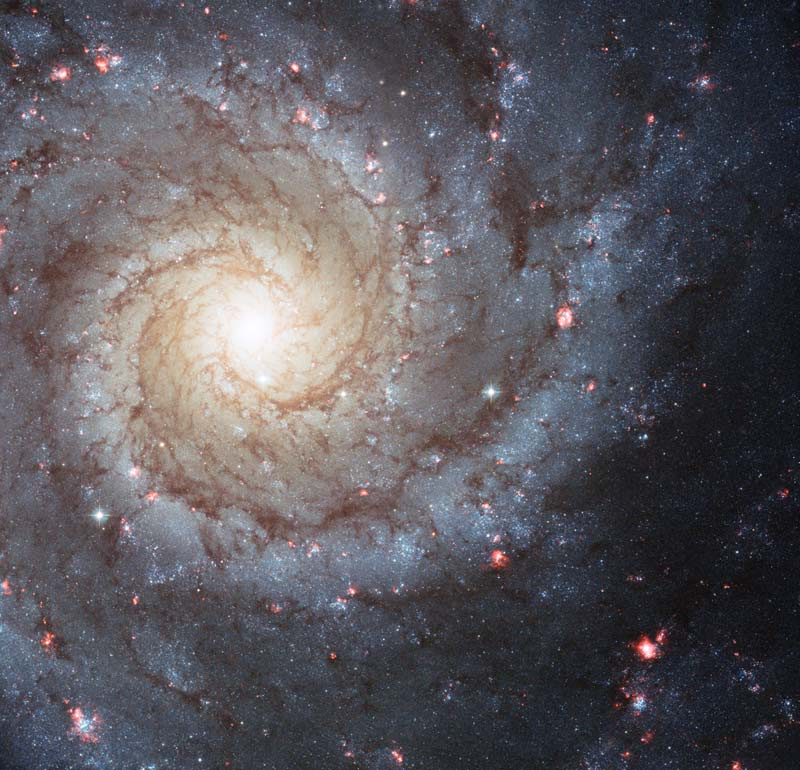
\includegraphics[scale=0.2]{chapters/test-models/img/ngc_628.jpg}
        \caption{Real-world spiral galaxy (NGC 3147).}
        \label{fig:ngc-628}
    \end{subfigure}

    \vspace{0.5em}
    {\footnotesize
        Credit for Figure~\ref{fig:ngc-628}: NASA, ESA, and the Hubble Heritage (STScI/AURA)-ESA/Hubble Collaboration;
        Acknowledgment: R. Chandar (University of Toledo) and J. Miller (University of Michigan). \par}

    \caption{Comparison between a modeled and a real-world spiral galaxy.}
    \label{fig:galaxy-comparison}
\end{figure}
\autoref{fig:ngc-628} shows an example of a real-world spiral galaxy whose general structure we aim to reproduce.

\subsection{Disk}\label{subsec:disk}
The disk particles are sampled from a radial distribution
\begin{equation*}
    p(r) = \frac{3}{\pi R_D^2}\left(1 - \frac{r}{R_D}\right), \; z = 0,
\end{equation*}
where $R_D$ is the radius of the disk and $r \leq R_D$.
The cumulative distribution function is therefore
\begin{equation*}
    F(r, \phi) = \int_{0}^{\phi}\int_{0}^{r} p(r') r'dr'd\phi' = \frac{\phi}{2\pi R_D^3}(3R_D r^2-2r^3)
\end{equation*}
and the marginal CDFs are
\begin{equation*}
    F_R(r) = F(r, 2\pi) = \frac{1}{R_D^3}(3R_D r^2-2r^3) \quad \text{and} \quad F_\Phi(\phi) = F(R_D, \phi) = \frac{\phi}{2\pi}.
\end{equation*}
Now we use inverse transform sampling to generate initial positions $(r, \phi)$ for the particles, i.e. $\phi = 2\pi u$ and $r$ is given implicitly by $h(r) \equiv 2r^3 - 3R_D r^2 + uR_D^3 = 0$ with $u \sim U(0, 1)$.
A straightforward calculation shows that $dh/dr < 0$ for $0 < r < R_D$ and $h(0)h(R_D) < 0$, implying that $h$ has exactly one zero between 0 and $R_D$ (which can be found for example using Newton's method).

Strength of the gravitational field $\mathbf{g}_D$ due to the disk at point $\mathbf{x}_0$ lying in the disk is
\begin{equation*}
    \mathbf{g}_D = G \int_{0}^{2\pi}\int_{0}^{R_D} \sigma(r) \frac{\mathbf{x} - \mathbf{x}_0}{|\mathbf{x} - \mathbf{x}_0|^3}r dr d\phi,
\end{equation*}
where $\sigma(r) = \sigma_0(1 - r/R_D)$ describes the density profile of the disk for $r \leq R_D$.
If $M_D$ is the total mass of the disk, then $\sigma_0 = 3M_D / (\pi R_D^2)$.
By symmetry, the point $\mathbf{x}_0$ may be chosen to lie on the $x$-axis, i.e. $\mathbf{x}_0 = (-x_0, 0)$, so that $\mathbf{x} - \mathbf{x}_0 = (x_0 + r\cos\phi, r\sin\phi)$.
Letting $\bar{r} = r/R_D$ and $\bar{x}_0 = x_0 / R_D$, the integral becomes
\begin{equation*}
    \mathbf{g}_D = G\sigma_0 \int_{0}^{2\pi} \int_{0}^{1} (1 - \bar{r}) \frac{(\bar{x}_0 + \bar{r}\cos\phi, \bar{r}\sin\phi)}{|(\bar{x}_0 + \bar{r}\cos\phi, \bar{r}\sin\phi)|^3}\bar{r} d\bar{r} d\phi.
\end{equation*}
By symmetry $g_{D,y} = 0$ and thus the radial component of the field $\mathbf{g}_D$ at distance $R\bar{x}_0$ from the center is
\begin{equation}\label{eq:gx-disk}
    g_{D,r} = -|\mathbf{g}_D| = -G\sigma_0 \int_{0}^{2\pi} \int_{0}^{1} (1 - \bar{r})\frac{\bar{x}_0 + \bar{r}\cos\phi}{(\bar{x}_0^2+\bar{r}^2+2\bar{x}_0\bar{r}\cos\phi)^{3/2}}\bar{r}d\bar{r}d\phi.
\end{equation}
If the disk had constant density, $\mathbf{g}_D$ could be expressed in terms of elliptic integrals \cite{Weiss2018}.
However, to the best of the author's knowledge, the integral in \autoref{eq:gx-disk} cannot be further simplified.
For this reason, a crude approximation with a quadratic function is used: $-g_{D,r} \approx a(r - h)^2 + k$, where the values $k=2.5$ and $h=0.66$ (the maximum of $g_{D,r}$ and the argument thereof) were estimated based on the graph of $g_{D,r}$ (see \autoref{fig:radial-strength-disk}).
The value of $a = -k/h^2$ can be found by setting $g_{D,r}(0) = 0$ in the approximate formula.
\begin{figure}[htp]
    \centering
    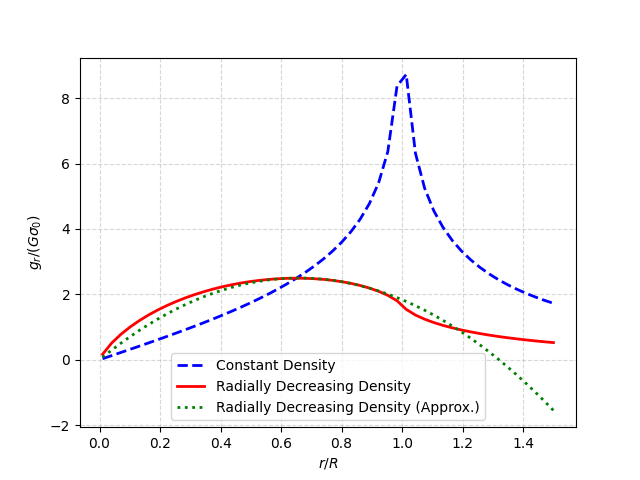
\includegraphics[scale=0.6]{chapters/test-models/img/disk-field.png}
    \caption{Magnitude of the radial component of the field strength due to a disk.
        The peak at $r=R$ for the constant density disk is, in fact, infinite.}
    \label{fig:radial-strength-disk}
\end{figure}

\subsection{Halo}
The density profile of the halo is analogous to the one used for the disk, save for the fact it is 3-dimensional, i.e.
\begin{equation*}
    \rho(r) =
    \begin{cases}
        \rho_0\left(1 - \frac{r}{R_H}\right), & r \leq R_H        \\
        0,                                    & \text{otherwise},
    \end{cases}
\end{equation*}
where $R_H$ is the radius of the halo.
If we let $M_H$ be the mass of the halo, then $\rho_0 = 3M_H / (\pi R_H^3)$.
Application of Gauss's law shows that we have
\begin{equation*}
    g_{H,r} = -G M_H \times
    \begin{cases}
        \frac{r}{R_H^3}\left(4 - \frac{3r}{R_H}\right), & r \leq R_H        \\
        \frac{1}{r^2},                                  & \text{otherwise}.
    \end{cases}
\end{equation*}

\subsection{Initial conditions}
The total field $\mathbf{g} = \mathbf{g}_D + \mathbf{g}_H$ is used to find initial velocities for the particles with initial positions $(x, y, 0)$.
The formula for the centripetal force yields
\begin{equation*}
    \frac{v^2}{r} = -g_r
\end{equation*}
and thus
\begin{equation*}
    \mathbf{v} = \left(-v \frac{y}{r}, v\frac{x}{r}, 0\right)
\end{equation*}
with $v = \sqrt{- r g_r}$
for counter-clockwise rotation.

\subsection{Disk with a hole}\label{subsec:disk-with-hole}
While testing the implemented methods, we observed that for modeling systems comprising multiple galaxies, it may be beneficial to replace the fixed halo with a single massive particle.
In such a case, the simulation turns out to be stable if there are no particles in close vicinity to the galaxy center.
This means that the galactic disk ought to have a hole of radius $r_0$.
Using an approach analogous to the one used in \autoref{subsec:disk}, we obtain the following relations that can be used for sampling points $(\phi, r)$ in polar coordinates
\begin{equation*}
    \phi = 2\pi u \quad \text{ and } \quad 2(r^3 - r_0^3)-3R_D(r^2 - r_0^2) + (R_D-r_0)^2(2r_0 + R_D)u = 0,
\end{equation*}
where $u \sim U(0, 1)$.

Getting rid of the external halo field simplifies the treatment of complex systems significantly, as we do not need to keep track of the movement of the halo.
The massive particle in the galaxy center, which effectively replaces it, can be treated just as any other particle in the simulation.
\section{Globular cluster model}\label{sec:globular-cluster-model}
A globular cluster is a formation comprising a large number of stars, closely packed in a spherically symmetric form \cite{britannica2024globular} (see \autoref{fig:messier-13}).
\begin{figure}[!ht]
    \centering
    \begin{subfigure}[b]{0.4\textwidth}
        \centering
        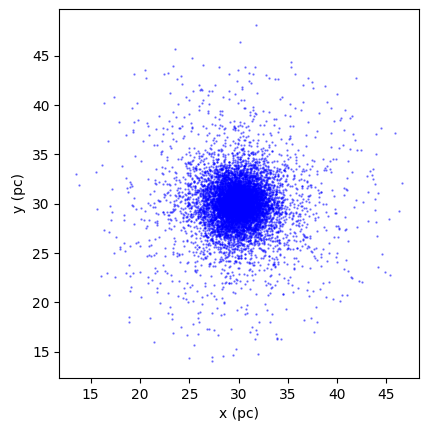
\includegraphics[width=\textwidth]{chapters/test-models/img/globular_generated.png}
        \caption{Generated data ($M=10^{6} M_\odot$, $a=2$ pc, $N=10,000$).}
        \label{fig:glob-cluster-model-generated}
    \end{subfigure}
    \hfill
    \begin{subfigure}[b]{0.4\textwidth}
        \centering
        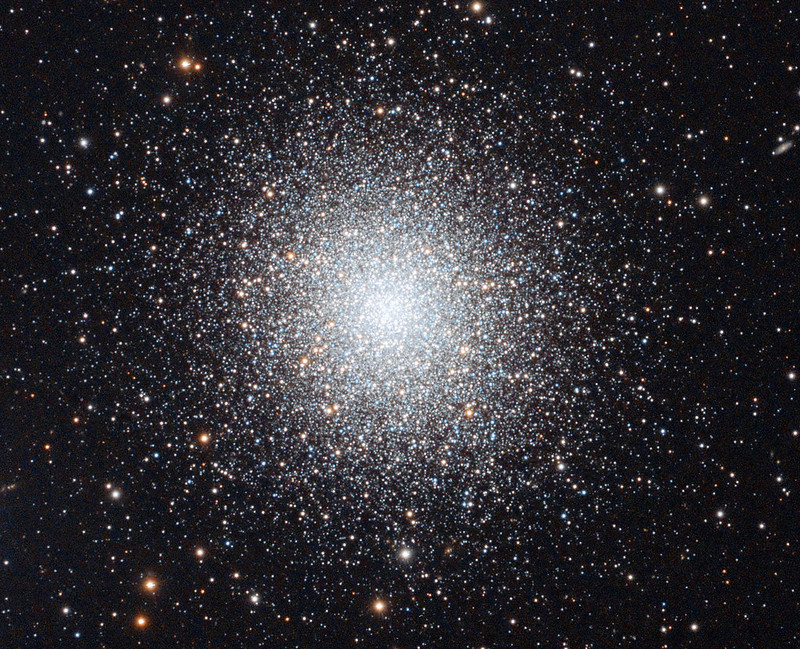
\includegraphics[width=\textwidth]{chapters/test-models/img/glob_cluster_m13.jpg}
        \caption{Real-world globular cluster (Messier 13).}
        \label{fig:messier-13}
    \end{subfigure}

    \vspace{0.5em}
    {\footnotesize
        Credit for Figure~\ref{fig:messier-13}: Giuseppe Donatiello. \par}

    \caption{The particle positions generated using the described model compared to a real-world globular cluster.}
    \label{fig:globular-cluster-gen-vs-real}
\end{figure}
In this work, we employed the implemented methods to simulate such a structure using the Plummer model.
This model was selected for its simplicity and widespread use, as well as the abundance of detailed descriptions available in the literature.

In the Plummer model, the density of a cluster is given by
\begin{equation}\label{eq:plummer-dens}
    \rho(r) = \frac{3M}{4\pi a^2}\left(1 + \frac{r^2}{a^2} \right)^{-5/2},
\end{equation}
where the parameter $a$ controls the spread of the distribution (the size of the cluster core) \cite{Aarseth1974Comparison}.
Hence, the particles are sampled from a distribution with PDF $p(r) = \rho(r) / M$.
Similarly to the galaxy model, we use inverse transform sampling to initialize the positions of the particles.
The marginal CDFs are easily calculated as
\begin{equation*}
    F_R(r) = \frac{r^3}{a^3}\left( 1+\frac{r^2}{a^2} \right)^{-3/2}, \quad
    F_\Theta (\theta) = \frac{1}{2}(1-\cos\theta), \quad
    F_\Phi (\phi) = \frac{\phi}{2\pi},
\end{equation*}\
which means that given a random variable $u\sim U(0, 1)$, we can generate random points with spherical coordinates
\begin{equation}\label{eq:plummer-random-init-pos}
    r = a(u^{-2/3}-1)^{-1/2}, \quad \theta = \cos^{-1}(1-2u), \quad \phi = 2\pi u,
\end{equation}
consistent with \autoref{eq:plummer-dens} (assuming equal mass of all particles).

In the Plummer model, the gravitational potential is given by
\begin{equation*}
    \phi(r) = -\frac{GM}{\sqrt{r^2 + a^2}}.
\end{equation*}
This expression can be used to determine the escape velocity \( v_e \) at a distance \( r \) from the center of the system.
Using the law of conservation of energy, we get
\begin{equation*}
    \frac{1}{2}v_e + \phi(r) = 0 \Rightarrow v_e = \sqrt{-2\phi(r)}.
\end{equation*}
For any $r$, the probability distribution of $q \equiv v/v_e$ is given by \cite{Aarseth1974Comparison}
\begin{equation}\label{eq:velocity-pdf}
    g(q) = N q^2(1-q^2)^{7/2},
\end{equation}
where $N$ is a normalization constant, which can be calculated to be $N = 512 / (7\pi)$.
The CDF of the distribution in \autoref{eq:velocity-pdf}, $G(q) = \int_0^q g(q') dq'$, can be determined using symbolic integration.
The algebraic expression that one obtains in this way is lengthy, and we will not cite it here.
The random values of $q$, consistent with the PDF in \autoref{eq:velocity-pdf}, are again obtained using inverse transform sampling;
the equation $G(q) = u$ is solved for $q$ by finding the roots of $G(q) - u$ using Newton's method.
Finally, the magnitude $v$ of the velocity vector $\mathbf{v}$ is set to $v = qv_e$.
The direction of $\mathbf{v} = (v_x, v_y, v_z)$ is chosen uniformly at random, i.e.
\begin{equation*}
    v_x = v\sin\theta \cos\phi, \quad v_y = v\sin\theta\sin\phi, \quad v_z = v\cos\theta,
\end{equation*}
where $\theta$ and $\phi$ are generated in the same way as in \autoref{eq:plummer-random-init-pos}.

The comparison of particle positions generated using the method above with an example of a real-world globular cluster is shown in \autoref{fig:globular-cluster-gen-vs-real}.

\chapter{Results}
All implemented methods were applied to three scenarios:
\begin{enumerate}
    \item Spiral galaxy simulation (\autoref{sec:galaxy-model}),
    \item Globular cluster simulation (\autoref{sec:globular-cluster-model}),
    \item Galaxy collision simulation (two galaxies modelled as ``disks with holes'', \autoref{subsec:disk-with-hole}).
\end{enumerate}
The choice of these scenarios hopefully well illustrates the versatility of the the methods introduced over the last couple of sections.

\section{Spiral galaxy simulation}\label{sec:spiral-galaxy-sim}
The parameters used in the simulation of a spiral galaxy are shown in \autoref{tab:galaxy-parameters}.
\begin{table}[htp]
    \centering
    \caption{Galaxy model parameters used in the simulation.}
    \label{tab:galaxy-parameters}
    \begin{tabular}{lc}
        \toprule
        \textbf{Parameter}   & \textbf{Value}           \\
        \midrule
        Halo radius          & 3 kpc                    \\
        Halo mass            & $60 \times 10^9 M_\odot$ \\
        Disk radius          & 15 kpc                   \\
        Disk mass            & $15 \times 10^9 M_\odot$ \\
        Disk thickness       & 0.3 kpc                  \\
        Disk density profile & Uniformly decreasing     \\
        \bottomrule
    \end{tabular}
\end{table}
The galaxy is simulated as an isolated system; however, in deriving \autoref{eq:poisson-fourier-product}, periodic boundary conditions were assumed.
The simplest way (and the one used) to obtain a free-space solution from the PM method is to extend the computational domain twice in every dimension and fill the space unused in mass distribution with zeros.
The total size of the potential mesh used was $128 \times 128 \times 64$ with the region of interest occupying a box of size $60\, \text{kpc}\times 60\, \text{kpc}\times 30\, \text{kpc}$ located in a $64 \times 64 \times 32$ octant of the mesh.

\subsection{PM method}
In the PM method, $N=50{,}000$ particles were used.
Cell size $H$ and timestep length were set to $60/64=0.9375$ kpc and 1 Myr, respectively.
For convenience, the full configuration of the PM method is presented in \autoref{tab:pm-method-parameters}.
\begin{table}[htp]
    \centering
    \caption{PM method configuration.}
    \label{tab:pm-method-parameters}
    \begin{tabular}{lc}
        \toprule
        \textbf{Parameter}      & \textbf{Value}                     \\
        \midrule
        Effective mesh size     & $64 \times 64 \times 32$           \\
        $H$ (cell size)         & $60/64=0.9375$ kpc                 \\
        DT (time step)          & $1$ Myr                            \\
        Mass assignment scheme  & TSC                                \\
        Finite difference       & Two-point                          \\
        Green's function        & Derived from discretized Laplacian \\
        Time integration method & Leapfrog                           \\
        Number of particles     & 50,000                             \\
        \bottomrule
    \end{tabular}
\end{table}
The system's evolution over 200 Myr is shown in \autoref{fig:spiral-galaxy-evolution-pm}.

\begin{figure}[!ht]
    \centering
    \begin{subfigure}[b]{0.45\textwidth}
        \centering
        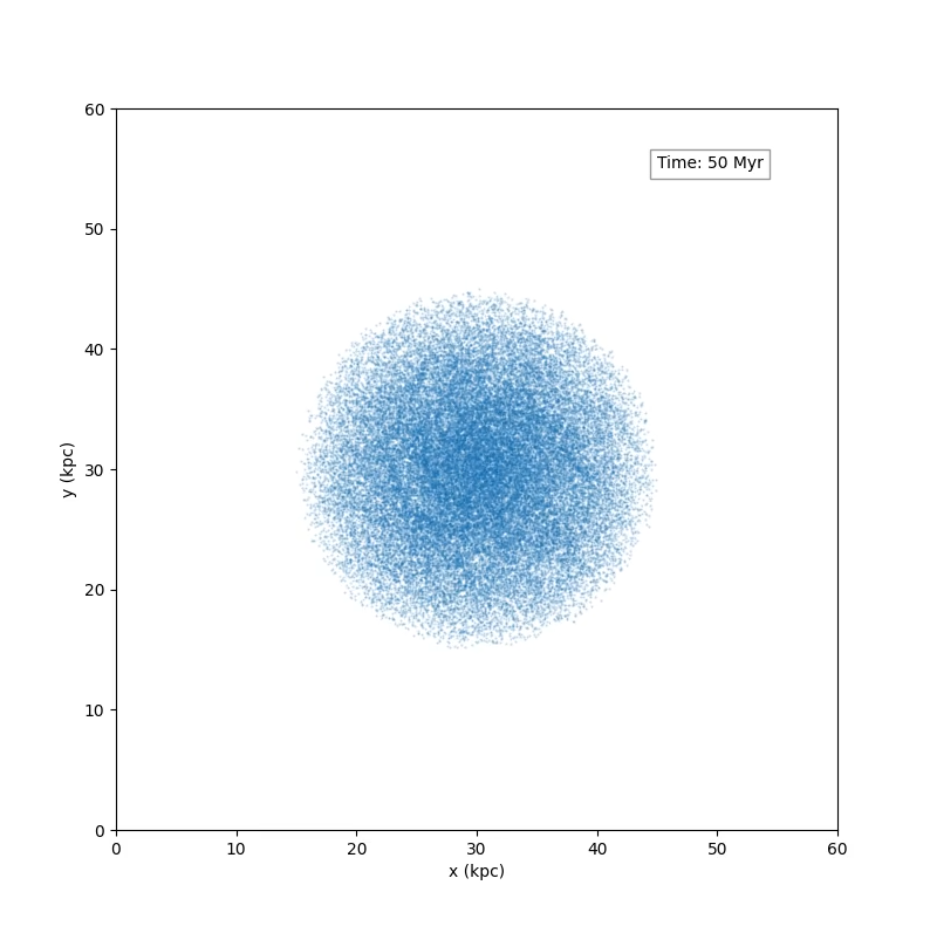
\includegraphics[width=\textwidth]{chapters/results/img/pm-galaxy/50myr.png}
        \caption{$t=50\,\text{Myr}$}
        \label{fig:spiral-galaxy-evolution-pm-sub1}
    \end{subfigure}
    \hfill
    \begin{subfigure}[b]{0.45\textwidth}
        \centering
        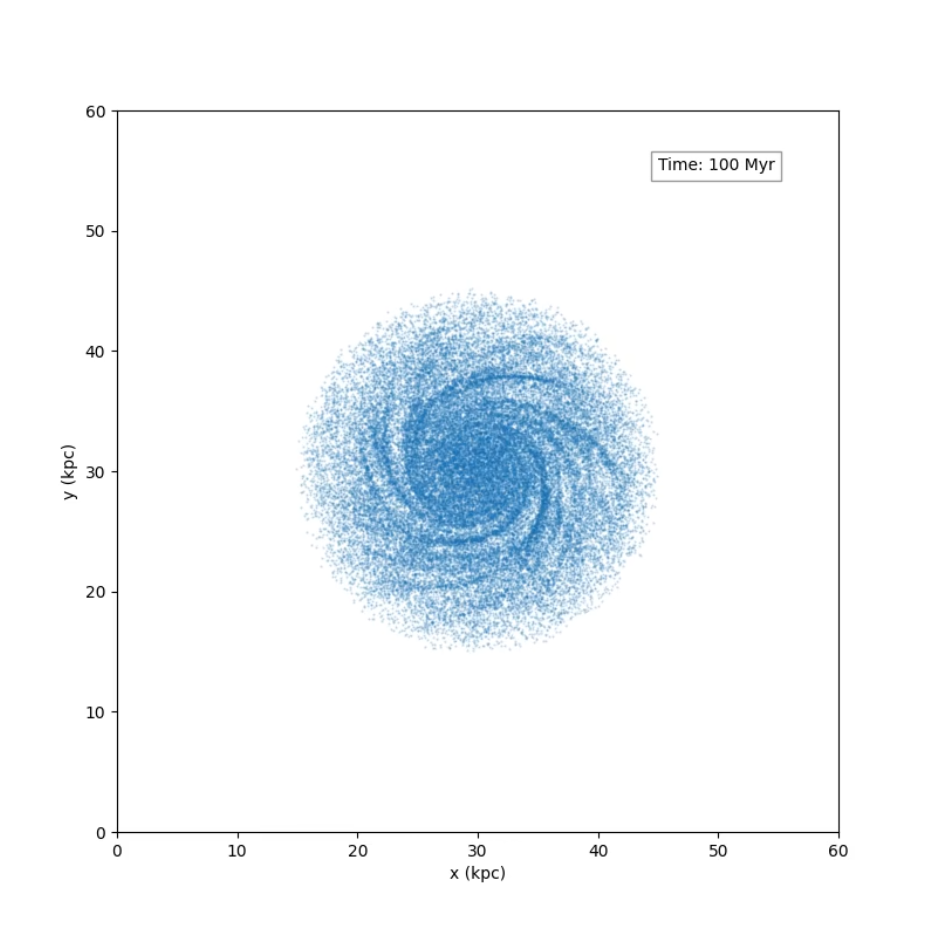
\includegraphics[width=\textwidth]{chapters/results/img/pm-galaxy/100myr.png}
        \caption{$t=100\,\text{Myr}$}
        \label{fig:spiral-galaxy-evolution-pm-sub2}
    \end{subfigure}

    \vspace{0.2cm}

    \begin{subfigure}[b]{0.45\textwidth}
        \centering
        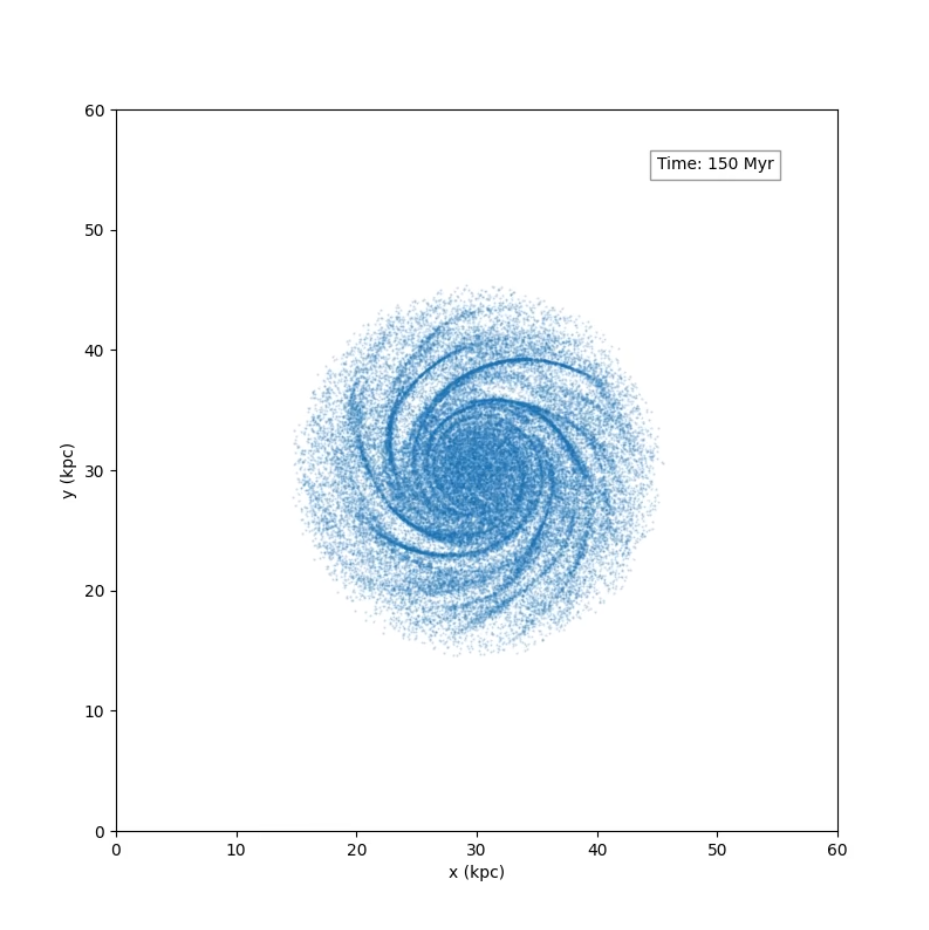
\includegraphics[width=\textwidth]{chapters/results/img/pm-galaxy/150myr.png}
        \caption{$t=150\,\text{Myr}$}
        \label{fig:spiral-galaxy-evolution-pm-sub3}
    \end{subfigure}
    \hfill
    \begin{subfigure}[b]{0.45\textwidth}
        \centering
        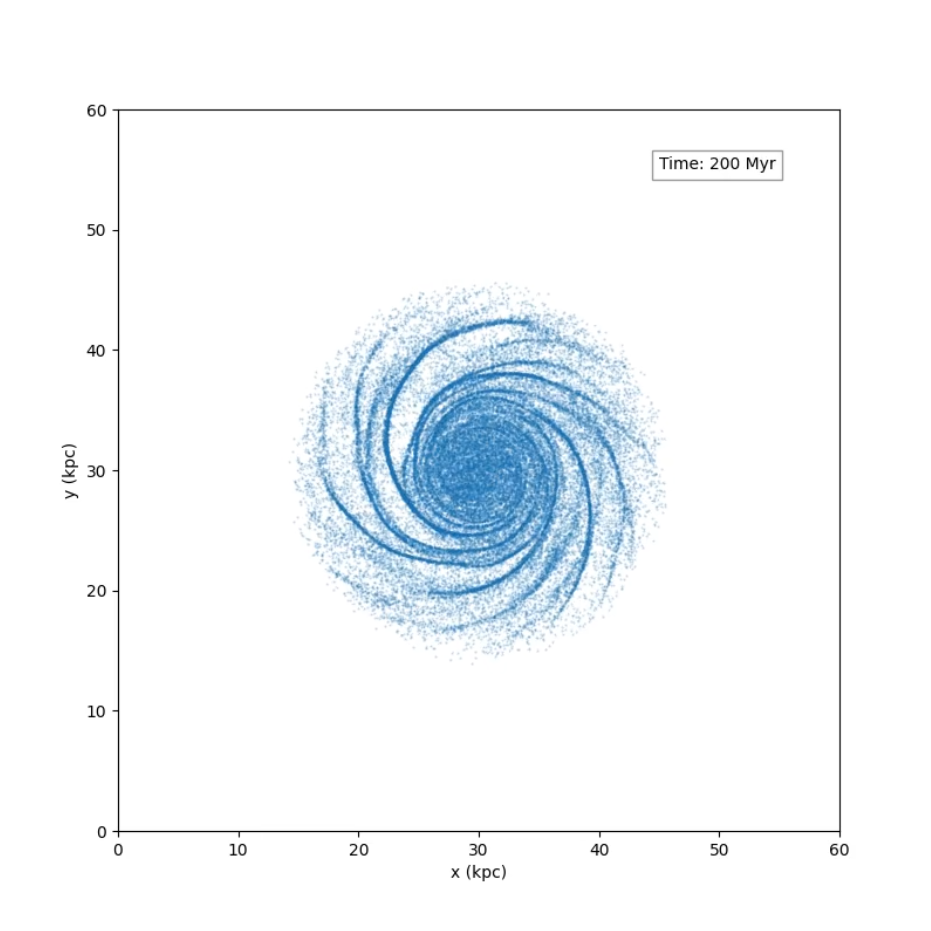
\includegraphics[width=\textwidth]{chapters/results/img/pm-galaxy/200myr.png}
        \caption{$t=200\,\text{Myr}$}
        \label{fig:spiral-galaxy-evolution-pm-sub4}
    \end{subfigure}

    \caption{Evolution of a spiral galaxy as predicted by the PM method.}
    \label{fig:spiral-galaxy-evolution-pm}
\end{figure}

During the simulation, total energy $E = \textrm{KE} + \textrm{PE}$, angular momentum $\mathbf{l}$, and the $z$-component of the momentum vector $\mathbf{p}$ should stay constant.
The $x$- and $y$-components of momentum change due to the presence of an external gravitational field (representing the halo) that exerts force $\mathbf{F}^\text{ext}$ on the system.
We can verify if this variation satisfies the expected relation
\begin{equation}\label{eq:expected-momentum-change}
    \dot{\mathbf{p}} = \mathbf{F}^\text{ext}
\end{equation}
by finding the initial total momentum $\mathbf{p}(t = 0)$ and incrementing the value of $\mathbf{p}$ in each time-step by $\mathbf{F}^\text{ext}\textrm{DT}$.

The exact calculation of the potential energy \cite{taylor2005classical} using the formula
\begin{equation*}
    \textrm{PE} = -\sum_{i=1}^{N}\sum_{j=i+1}^{N}\frac{G m_i m_j}{r_{ij}}
\end{equation*}
is computationally infeasible considering the $O(N^2)$ cost.
An approximation based on the potential values at mesh points,
\begin{equation*}
    \textrm{PE} \approx \frac{V}{2}\sum_{\mathbf{p}} \rho(\mathbf{x}_\mathbf{p})\phi(\mathbf{x}_\mathbf{p}),
\end{equation*}
is used instead (for derivation, refer to \cite{Hockney1988}).
\begin{figure}[!ht]
    \centering
    \begin{subfigure}[b]{0.45\textwidth}
        \centering
        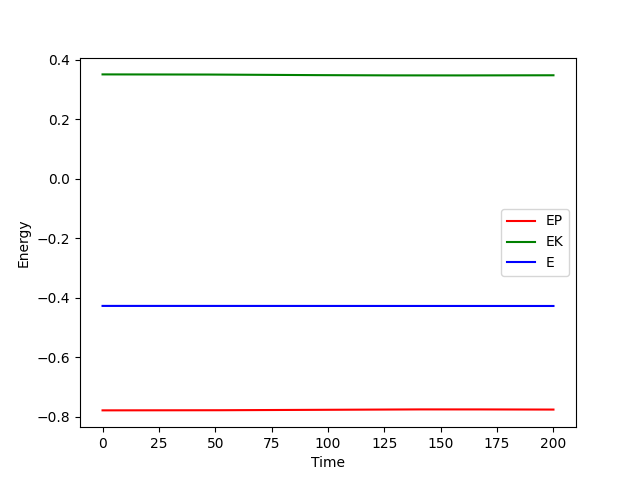
\includegraphics[width=\textwidth]{chapters/results/img/pm-galaxy/energy.png}
        \caption{Energy}
        \label{fig:physical-quantities-pm-sub1}
    \end{subfigure}
    \hfill
    \begin{subfigure}[b]{0.45\textwidth}
        \centering
        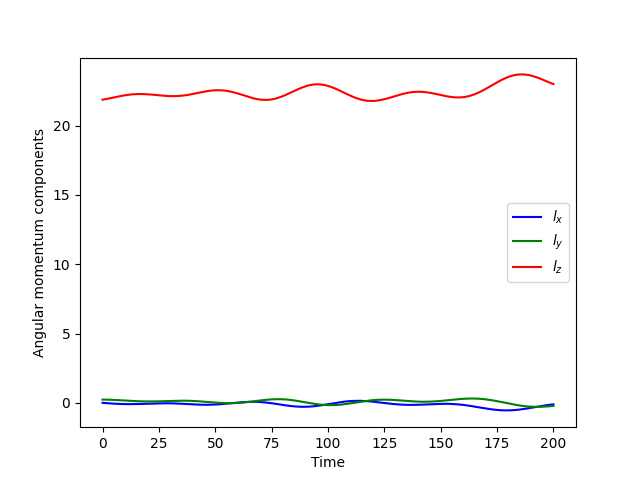
\includegraphics[width=\textwidth]{chapters/results/img/pm-galaxy/angular-momentum.png}
        \caption{Angular momentum}
        \label{fig:physical-quantities-pm-sub2}
    \end{subfigure}

    \vspace{0.2cm}

    \begin{subfigure}[b]{0.45\textwidth}
        \centering
        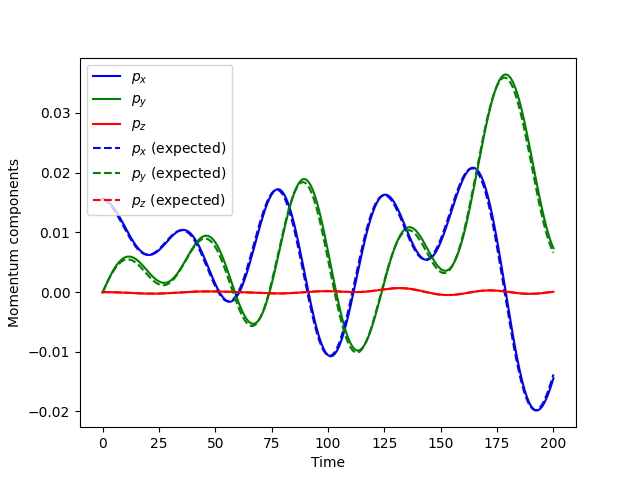
\includegraphics[width=\textwidth]{chapters/results/img/pm-galaxy/momentum.png}
        \caption{Momentum; broken lines represent the expected momentum following \autoref{eq:expected-momentum-change}}
        \label{fig:physical-quantities-pm-sub3}
    \end{subfigure}

    \caption{Fundamental physical quantities describing the system over time in the PM simulation.
        Time is in Myr, and the quantities are expressed in units consistent with \autoref{tab:galaxy-parameters}}
    \label{fig:physical-quantities-pm}
\end{figure}

\subsection{\texorpdfstring{\PThreeM{}}{P3M} method}
The \PThreeM{}-based simulation uses the same parameters as the PM method.
The reference force was calculated using the $S_1$ shape formula (\autoref{eq:s1-reference-force}) with particle diameter $a=3H$.
The cutoff radius was set to $r_e=0.7a$.
One extra free parameter is the \textit{softening length} $\epsilon$, which modifies the universal law of gravitation so that division by zero can be avoided, i.e., the modified law is
\begin{equation*}
    F^\text{soft}_{ij}(r) = \frac{G m_i m_j}{r_{ij}^2 + \epsilon^2}.
\end{equation*}
In the simulation, $\epsilon$ was set arbitrarily to $1.5$ kpc.
The whole configuration of the \PThreeM{} method is conveniently shown in \autoref{tab:p3m-method-parameters}.
The system's evolution is presented in \autoref{fig:spiral-galaxy-evolution-p3m}, and the graphs of energy, angular momentum, and momentum components vs. time are shown in \autoref{fig:physical-quantities-p3m}.

\subsection{Barnes-Hut algorithm}
For the Barnes-Hut algorithm test, the initial conditions of the system remain the same as in the two previous simulations.
The softening length $\epsilon$ was set to 1 kpc, and quadrupole terms were omitted.
The whole configuration of the method is shown in \autoref{tab:bh-method-parameters}.
The snapshots of the simulation are displayed in \autoref{fig:spiral-galaxy-evolution-bh}, and the graphs showing how the energy, momentum, and angular momentum varied over time are shown in \autoref{fig:physical-quantities-bh}.

\subsection{Commentary}
All of the implemented methods successfully reproduced the expected structural features of a spiral galaxy.
A region of high density is clearly localized in the center of the galaxy, and characteristic spiral arms emerge around the 150 Myr mark.
The snapshots from all three simulations (\autoref{fig:spiral-galaxy-evolution-pm}, \autoref{fig:spiral-galaxy-evolution-p3m}, and \autoref{fig:spiral-galaxy-evolution-bh}) show similar evolution of the system over time, with the last snapshot of each simulation visually resembling a real-world spiral galaxy (cf. \autoref{fig:ngc-628}).
It is worth noting, however, that the system evolves more rapidly in the PM-based simulation.
For instance, the spiral arms are significantly more developed at $t = 100$ Myr (\autoref{fig:spiral-galaxy-evolution-pm-sub2}) compared to the same time point in the simulations using the other two methods.
This accelerated evolution is likely due to the smaller ``induced softening length'' inherent to the PM method, which results in stronger gravitational forces. These limitations were anticipated and discussed in \autoref{subsubsec:pm-global-picture}.

Energy plots (\autoref{fig:physical-quantities-pm-sub1}, \autoref{fig:physical-quantities-p3m-sub1}, and \autoref{fig:physical-quantities-bh-sub1}) show that each of the methods tested conserved the total energy.
The plots of angular momentum over time (\autoref{fig:physical-quantities-pm-sub2}, \autoref{fig:physical-quantities-p3m-sub2}, and \autoref{fig:physical-quantities-bh-sub2}) illustrate that the angular momentum was \textit{on average} constant with the variations stemming from the presence of the external halo field.
Finally, the momentum plots (\autoref{fig:physical-quantities-pm-sub3}, \autoref{fig:physical-quantities-p3m-sub3}, and \autoref{fig:physical-quantities-bh-sub3}) demonstrate that the $z$-component of the momentum vector remains constant, while the remaining components change (again due to the external field).
The comparison of the actual values of the momentum with the theoretical values, updated in each timestep according to \autoref{eq:expected-momentum-change}, shows that the change in the $x$- and $y$-components is correct.

\section{Globular cluster simulation}
The globular cluster is simulated using the Plummer model with parameters set to the values in \autoref{tab:cluster-parameters}.
\begin{table}[htp]
    \centering
    \begin{tabular}{|l|c|}
        \hline
        \textbf{Parameter} & \textbf{Value}          \\
        \hline
        $a$ (spread)       & 2 pc                    \\
        Mass               & $1 \times 10^6 M_\odot$ \\
        Maximum radius     & 15 pc                   \\
        \hline
    \end{tabular}
    \caption{Galaxy model parameters used in the simulation.}
    \label{tab:cluster-parameters}
\end{table}
The \textit{maximum radius} parameter was introduced simply to confine the cluster to a predefined computational domain.
We restrict the presentation of our results to the simulation conducted using the Barnes-Hut algorithm, since other methods yielded very similar results.

\subsection{Barnes-Hut algorithm}
The configuration of the Barnes-Hut algorithm used in the globular cluster simulation is given in \autoref{tab:bh-method-parameters-cluster}.
\begin{table}[htp]
    \centering
    \begin{tabular}{|l|c|}
        \hline
        \textbf{Parameter}            & \textbf{Value} \\
        \hline
        $\theta$ (opening angle)      & 0.5            \\
        $\epsilon$ (softening length) & 0.5 pc         \\
        DT (time step)                & $1$ kyr        \\
        Highest multipole term        & quadrupole     \\
        \hline
    \end{tabular}
    \caption{Barnes-Hut method configuration.}
    \label{tab:bh-method-parameters-cluster}
\end{table}
The conservation of energy, momentum, and angular momentum during the simulation is demonstrated in \autoref{fig:physical-quantities-bh-cluster}.
\begin{figure}[htp]
    \centering
    \begin{subfigure}[b]{0.45\textwidth}
        \centering
        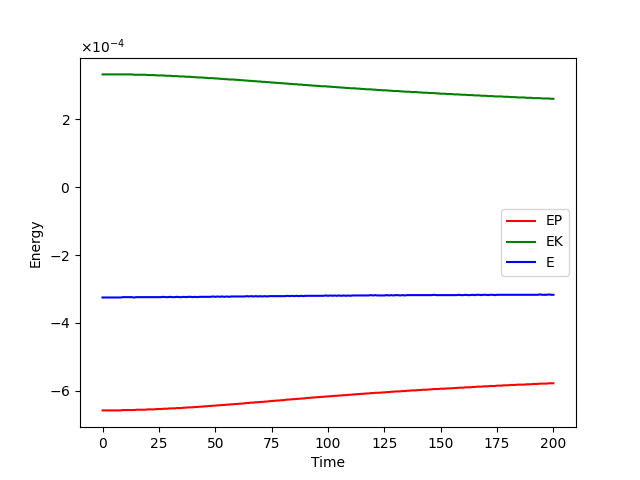
\includegraphics[width=\textwidth]{img/bh-cluster/energy.png}
        \caption{Energy}
        \label{fig:physical-quantities-bh-cluster-sub1}
    \end{subfigure}
    \hfill
    \begin{subfigure}[b]{0.45\textwidth}
        \centering
        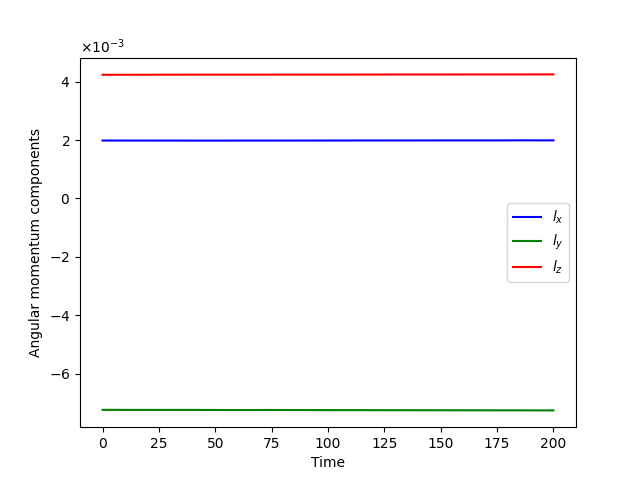
\includegraphics[width=\textwidth]{img/bh-cluster/angular-momentum.png}
        \caption{Angular momentum}
        \label{fig:physical-quantities-bh-cluster-sub2}
    \end{subfigure}

    \vspace{0.5cm}

    \begin{subfigure}[b]{0.45\textwidth}
        \centering
        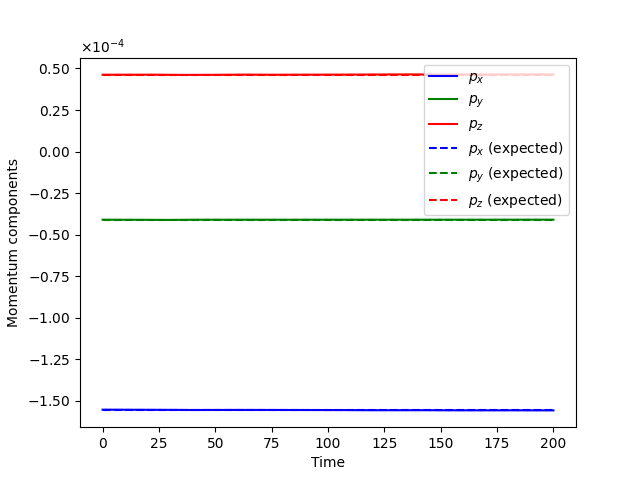
\includegraphics[width=\textwidth]{img/bh-cluster/momentum.png}
        \caption{Momentum; broken lines represent the expected momentum following \autoref{eq:expected-momentum-change}}
        \label{fig:physical-quantities-bh-cluster-sub3}
    \end{subfigure}

    \caption{Fundamental physical quantities describing the system over time in the Barnes-Hut algorithm.
        Time is in kyr and the quantities are expressed in units consistent with \autoref{tab:cluster-parameters}}
    \label{fig:physical-quantities-bh-cluster}
\end{figure}
Notice that the conservation of momentum and angular momentum is possible due to a lack of any external forces (this is contrasted with the previous test -- galaxy simulation with halo modelled a fixed, external field).
The evolution of the system (initial positions and after 200 kyr) is shown in \autoref{fig:cluster-evolution-bh}.
\begin{figure}[htp]
    \centering
    \begin{subfigure}[b]{0.45\textwidth}
        \centering
        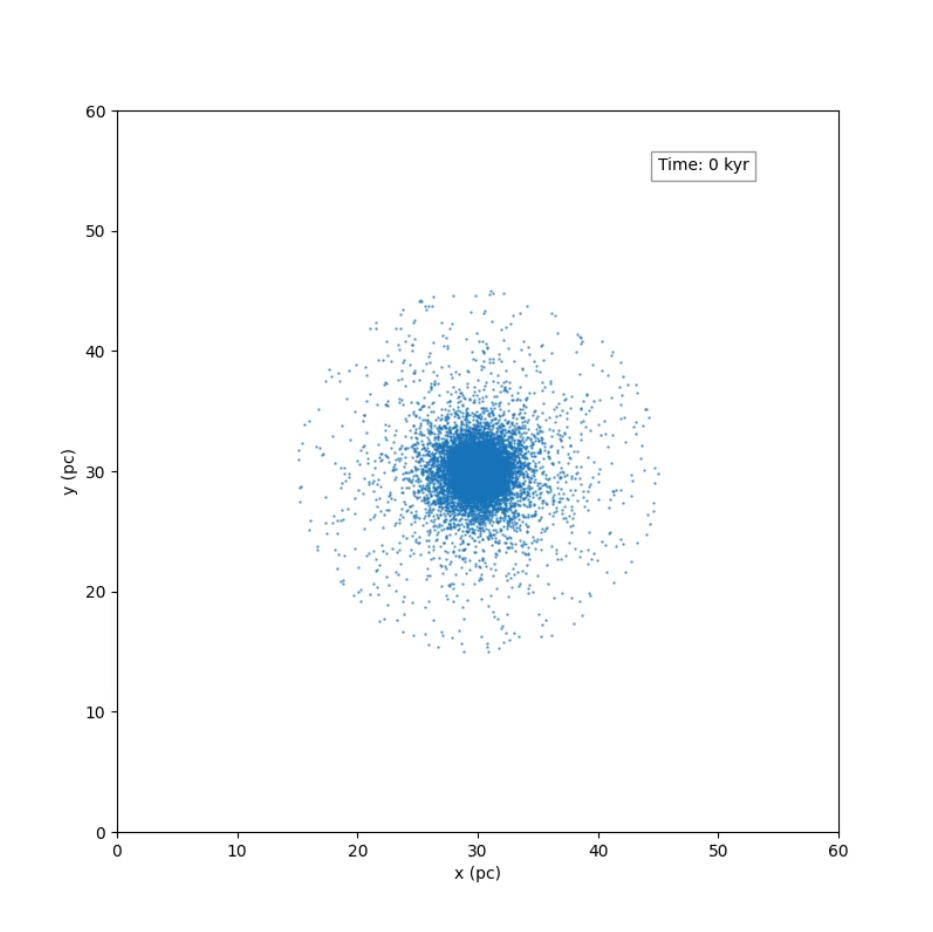
\includegraphics[width=\textwidth]{img/bh-cluster/0kyr.png}
        \caption{$t=0\,\text{kyr}$}
        \label{fig:cluster-evolution-bh-cluster-sub1}
    \end{subfigure}
    \hfill
    \begin{subfigure}[b]{0.45\textwidth}
        \centering
        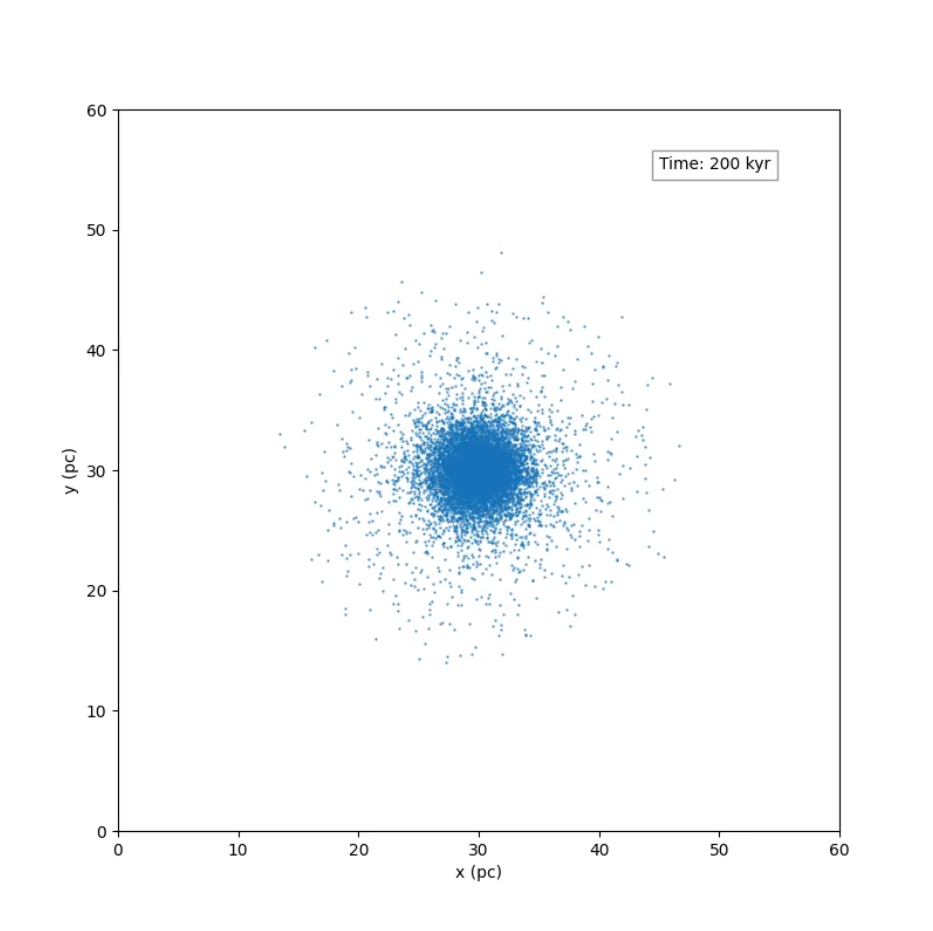
\includegraphics[width=\textwidth]{img/bh-cluster/200kyr.png}
        \caption{$t=200\,\text{kyr}$}
        \label{fig:cluster-evolution-bh-cluster-sub2}
    \end{subfigure}
    \caption{Evolution of a globular cluster as predicted by the Barnes-Hut algorithm.}
    \label{fig:cluster-evolution-bh}
\end{figure}
As can be seen, the system remains stable and bound gravitationally.
Also, in the initial snapshot (\autoref{fig:cluster-evolution-bh-cluster-sub1}) the effect of restricting the sampled points to a sphere of radius can be seen.
The system bears general resemblance to real-world globular clusters (cf. \autoref{fig:messier-13}).
\section{Galaxy collision simulation}
We conclude showcasing the applications of our program with a simulation of collision of two galaxies.
The parameters describing the galaxies are given in \autoref{tab:galaxy-parameters-collision}.
\begin{table}[htp]
    \centering
    \begin{tabular}{|l|c|c|}
        \hline
        \textbf{Parameter}   & \textbf{Galaxy 1}        & \textbf{Galaxy 2}        \\
        \hline
        Center position      & (40, 30, 15) kpc         & (80, 30, 15) kpc         \\
        Halo radius          & 3 kpc                    & 2 kpc                    \\
        Halo mass            & $60 \times 10^9 M_\odot$ & $40 \times 10^9 M_\odot$ \\
        Disk radius          & 15 kpc                   & 10 kpc                   \\
        Disk mass            & $15 \times 10^9 M_\odot$ & $10 \times 10^9 M_\odot$ \\
        Disk thickness       & 0.3 kpc                  & 0.3 kpc                  \\
        Disk density profile & Uniformly decreasing     & Uniformly decreasing     \\
        Number of particles  & $3 \times 10^4$          & $3 \times 10^4$          \\
        \hline
    \end{tabular}
    \caption{Galaxy model parameters used in the simulation.}
    \label{tab:galaxy-parameters-collision}
\end{table}
\subsection{Barnes-Hut algorithm}
The configuration of the algorithm is given in \autoref{tab:bh-method-parameters-collision}.
\begin{table}[htp]
    \centering
    \begin{tabular}{|l|c|}
        \hline
        \textbf{Parameter}            & \textbf{Value} \\
        \hline
        $\theta$ (opening angle)      & 1              \\
        $\epsilon$ (softening length) & 1.3 kpc        \\
        DT (time step)                & $1$ Myr        \\
        Simulation duration           & 400 Myr        \\
        Highest multipole term        & Monopole       \\
        \hline
    \end{tabular}
    \caption{Barnes-Hut method configuration.}
    \label{tab:bh-method-parameters-collision}
\end{table}



% \subsection{Performance analysis}
% The PM and \PThreeM{} methods were implemented exactly as described in the previous sections.
% The PM method was developed for both CPU and GPU architectures, using C++ and CUDA C++, respectively.
% The implementation relies on external libraries for fast Fourier transform computations: FFTW for the CPU version and cuFFT for the GPU version.
% A performance comparison of the PM method was conducted with $N$ ranging between 50,000 and 1,000,000 over 200 iterations (TSC mass assignment and two-point finite difference).
% The tests were run on a system equipped with an Intel(R) Core(TM) i7-9750H CPU @ 2.60GHz and an NVIDIA GeForce GTX 1650 GPU.
% For the purposes of performance evaluation, the parts of the code responsible for diagnostics collection (energy, momentum, etc.) were switched off.
% Since disk IO (saving simulation state) was the most time-consuming part of both the CPU and GPU implementation, only the final state of the simulation was saved in these tests.
% This means that data transfers from device to host were also not taken into account.
% The results of the test are displayed in \autoref{fig:cpu-vs-gpu-pm}.


% For the \PThreeM{} method, performance was measured using $N=50,000$ particles on a $128 \times 128 \times 64$ mesh with the TSC assignment scheme.
% The total runtime was approximately 1 minute and 30 seconds, with the time distribution among key algorithm components as follows:
% \begin{itemize}
%     \item HOC table initialization: 12\%
%     \item Short-range force calculations: 80\%
%     \item PM step: 7.5\%
% \end{itemize}
% The code is available at \url{https://github.com/AleksyBalazinski/ParticleSimulation} under the MIT license.

\bibliographystyle{plain}
\bibliography{refs}


\end{document}